% =====================================================================
%  Data-Center GPU Platforms Compared  --  a lecture comparing NVIDIA's
%  platforms from the A100 to Vera Rubin with AMD's Instinct line
%  (MI100 to MI450 and the Helios rack) and Intel's GPUs (the Gen
%  graphics families, Xe-HPC Ponte Vecchio and Aurora, Xe2/Xe3, Gaudi,
%  and what follows): architecture, memory, interconnect, software
%  stacks, systems and measured results.
%  Same visual language as "Introduction to GPU Architectures".
%
%  Compile:  pdflatex gpu_platforms_compared_tutorial.tex   (run twice)
%  Self-contained: every figure is TikZ/pgfplots source in this file.
%
%  Conventions
%   * \stage{n} before a frame sets the accent color and highlights the
%     matching chip in the footer strip.
%   * Numbers quoted from a paper or a vendor report name the source;
%     numbers labeled "derived" were computed from quoted ones; curves
%     labeled "illustrative" are sketches, not data; $^\dagger$ marks
%     vendor documentation, model cards, blogs and commentary.
% =====================================================================
\documentclass[aspectratio=169,11pt]{beamer}

% ---------- fonts ----------------------------------------------------
\usepackage[scaled=0.92]{helvet}        % Helvetica-like sans for text
\renewcommand{\ttdefault}{cmtt}         % Computer Modern mono for tokens
\usefonttheme[onlymath]{serif}          % classic serif math
\usepackage{amsmath,amssymb,bm}
\usepackage{booktabs,array}
\usepackage{graphicx}


% ---------- graphics -------------------------------------------------
\usepackage{tikz}
\usepackage{pgfplots}
\pgfplotsset{compat=1.17}
\usetikzlibrary{arrows.meta,positioning,calc,fit,backgrounds,
                decorations.pathreplacing,shapes.geometric}

% ---------- palette --------------------------------------------------
\definecolor{ink}{HTML}{1F2937}     % text, residual stream
\definecolor{muted}{HTML}{6B7280}   % secondary text
\definecolor{hair}{HTML}{D9DDE4}    % hairlines
\definecolor{paper}{HTML}{FCFCFA}   % slide background
\definecolor{tok}{HTML}{5F6F85}     % tokens / tokenizer
\definecolor{emb}{HTML}{0CA678}     % embeddings
\definecolor{posc}{HTML}{7048E8}     % positional information
\definecolor{attn}{HTML}{E8590C}    % attention
\definecolor{mlp}{HTML}{1C7ED6}     % MLP / feed-forward
\definecolor{norm}{HTML}{5C940D}    % normalization
\definecolor{outc}{HTML}{D6336C}     % unembedding / softmax / sampling
\definecolor{trn}{HTML}{9C6644}     % training and scaling
\colorlet{qc}{attn}                 % queries
\definecolor{kc}{HTML}{F59F00}      % keys
\definecolor{vc}{HTML}{1098AD}      % values
\colorlet{kct}{kc!70!black}         % key color, darkened for text
\colorlet{stagec}{ink}              % accent of the current stage

% ---------- beamer look ----------------------------------------------
\setbeamertemplate{navigation symbols}{}
\setbeamercolor{background canvas}{bg=paper}
\setbeamercolor{normal text}{fg=ink}
\setbeamercolor{frametitle}{fg=ink}
\setbeamersize{text margin left=8mm,text margin right=8mm}
\setbeamertemplate{itemize item}{\raisebox{0.25ex}{\tiny\color{stagec}$\blacksquare$}}
\setlength{\leftmargini}{1.1em}
\hyphenpenalty=10000 \exhyphenpenalty=10000   % no hyphenation on slides

% stage = which part of the pipeline the slide belongs to
\newcount\stageno \stageno=1
\newcommand{\stage}[1]{\global\stageno=#1\relax
  \ifcase#1\or\colorlet{stagec}{ink}\or\colorlet{stagec}{tok}%
  \or\colorlet{stagec}{emb}\or\colorlet{stagec}{attn}%
  \or\colorlet{stagec}{mlp}\or\colorlet{stagec}{posc}%
  \or\colorlet{stagec}{trn}\or\colorlet{stagec}{outc}%
  \or\colorlet{stagec}{vc}\or\colorlet{stagec}{ink}\fi}

\makeatletter
% title: accent bar + title + one-line claim (the frame subtitle)
\setbeamertemplate{frametitle}{%
  \nointerlineskip\vspace*{3.6mm}%
  \begin{tikzpicture}[x=1mm,y=1mm]
    \useasboundingbox (0,0) rectangle (144,10.5);
    \fill[stagec,rounded corners=0.5mm] (0,0.3) rectangle (1.5,10.2);
    \ifx\insertframesubtitle\@empty
      \node[anchor=west,inner sep=0,text=ink,
            font=\fontsize{15}{17}\selectfont\bfseries] at (4.2,5.2) {\insertframetitle};
    \else
      \node[anchor=west,inner sep=0,text=ink,
            font=\fontsize{15}{17}\selectfont\bfseries] at (4.2,7.1) {\insertframetitle};
      \node[anchor=west,inner sep=0,text=muted,
            font=\fontsize{8.6}{10}\selectfont] at (4.2,2.0) {\insertframesubtitle};
    \fi
  \end{tikzpicture}}
\makeatother

% footer: pipeline strip with the current stage lit, plus page number
\setbeamertemplate{footline}{%
  
\begin{tikzpicture}[x=1mm,y=1mm]
    \useasboundingbox (0,0) rectangle (160,7.2);
    \coordinate (c0) at (7.2,4.0);
    \foreach \lab/\col [count=\i,remember=\i as \prev (initially 0)] in
      {Overview/ink,NVIDIA/tok,AMD/emb,Intel Gen/attn,Xe-HPC/mlp,
       Links/posc,Software/trn,Systems/outc,Benchmarks/vc,Wrap-up/ink}{
      \ifnum\i=\stageno
        \node[anchor=west,inner xsep=1.5mm,inner ysep=0.75mm,rounded corners=0.7mm,
              fill=\col,text=white,text height=1.5ex,text depth=0.35ex,
              font=\fontsize{5.8}{7}\selectfont\bfseries] (c\i) at ([xshift=0.8mm]c\prev.east) {\lab};
      \else
        \node[anchor=west,inner xsep=1.5mm,inner ysep=0.75mm,
              text=muted!80,text height=1.5ex,text depth=0.35ex,
              font=\fontsize{5.8}{7}\selectfont] (c\i) at ([xshift=0.8mm]c\prev.east) {\lab};
      \fi}
    \node[anchor=east,inner sep=0,text=muted,
          font=\fontsize{6.5}{8}\selectfont] at (152,4.0)
          {\insertframenumber\,/\,\inserttotalframenumber};
  \end{tikzpicture}}

% ---------- TikZ vocabulary ------------------------------------------
\tikzset{
  >={Stealth[length=4.6pt,width=4pt]},
  flow/.style={->,line width=0.8pt,draw=ink!70},
  thinflow/.style={->,line width=0.5pt,draw=ink!55},
  % component box (tinted) and its solid variant; argument = color
  comp/.style={rounded corners=2.2pt,draw=#1,fill=#1!12,line width=0.8pt,
               align=center,inner sep=4pt,font=\small,text=ink},
  fillbox/.style={rounded corners=2.2pt,fill=#1,text=white,align=center,
                inner sep=4pt,font=\small\bfseries},
  % a token
  chip/.style={rounded corners=1.8pt,fill=tok!14,draw=tok!55,line width=0.5pt,
               font=\ttfamily\footnotesize,inner xsep=3.5pt,inner ysep=2.5pt,
               text height=1.5ex,text depth=0.45ex,text=ink},
  cchip/.style={chip,fill=#1!16,draw=#1!75},
  lab/.style={font=\scriptsize,text=muted,inner sep=1.5pt},
  txt/.style={font=\footnotesize,text=ink,align=flush left,inner sep=0pt},
  plus/.style={circle,draw=ink,fill=paper,line width=0.75pt,inner sep=0pt,
               minimum size=9.5pt,font=\scriptsize\bfseries},
  brace/.style={decorate,decoration={brace,amplitude=3.5pt},draw=muted,line width=0.6pt},
}

% \cells{x}{y}{size}{color}{shade,shade,...}: a row of vector cells
\newcommand{\cells}[5]{%
  \foreach \sh [count=\ci from 0] in {#5}{%
    \fill[#4!\sh!white,draw=paper,line width=0.4pt]
      ({#1+\ci*#3},{#2}) rectangle ++(#3,#3);}}

% \rgrid{x}{y}{rows}{cols}{size}{color}{seed}: a matrix with varied shading
\newcommand{\rgrid}[7]{%
  \foreach \ri in {1,...,#3}{\foreach \ci in {1,...,#4}{%
    \pgfmathtruncatemacro\sh{16+mod(\ri*37+\ci*53+\ri*\ci*11+#7*29,8)*10}%
    \fill[#6!\sh!white,draw=paper,line width=0.4pt]
      ({#1+(\ci-1)*#5},{#2+(#3-\ri)*#5}) rectangle ++(#5,#5);}}}

% \barh{x}{y}{length}{color}: one horizontal bar of a bar chart
\newcommand{\barh}[4]{\fill[#4,rounded corners=0.8pt] ({#1},{#2-0.13}) rectangle ++({#3},0.26);}

% \valgrid{x}{y}{size}{color}{scale}{mask}{\rows}: matrix shaded by value.
% (x,y) is the top-left corner; \rows is a macro holding {a,b,..},{..},..
% With mask=1 the cells above the diagonal are drawn as blocked.
\newcommand{\valgrid}[7]{%
  \edef\vglist{#7}%
  \foreach \row [count=\r from 0] in \vglist {\foreach \v [count=\c from 0] in \row {%
    \pgfmathtruncatemacro\sh{min(100,\v*#5)}%
    \pgfmathtruncatemacro\msk{and(#6>0,\c>\r)}%
    \ifnum\msk=1
      \fill[tok!10,draw=paper,line width=0.4pt] ({#1+\c*#3},{#2-(\r+1)*#3}) rectangle ++(#3,#3);
    \else
      \fill[#4!\sh!white,draw=paper,line width=0.4pt] ({#1+\c*#3},{#2-(\r+1)*#3}) rectangle ++(#3,#3);
    \fi}}}

% the running attention example: Alice thanked Bob because she
\def\Sraw{{2.0,0.7,1.3,0.4,1.1},{1.8,1.2,0.9,1.6,0.5},{0.6,1.5,1.9,0.8,1.4},
          {0.8,1.6,0.9,1.1,2.1},{3.1,0.9,1.4,1.0,1.5}}          % scores
\def\Aw{{1.00,0,0,0,0},{.65,.35,0,0,0},{.14,.35,.51,0,0},
        {.18,.39,.19,.24,0},{.62,.07,.11,.08,.12}}              % softmax rows

% paper figure: \paperfig{file}{width}{Figure n}
\newcommand{\paperfig}[3]{%
  \begin{tikzpicture}
    \node[inner sep=0] (img) {\includegraphics[width=#2]{#1}};
    \node[anchor=north east,font=\fontsize{5.5}{6}\selectfont,text=muted,
          rounded corners=1pt,fill=ink!6,inner sep=2pt] at ([xshift=-1mm,yshift=-1mm]img.north east) {report, #3};
  \end{tikzpicture}}
% background panel: \bgpanel{x}{y}{width}{title}{body}  (anchor north west)
\newcommand{\bgpanel}[5]{%
  \node[anchor=north west,inner sep=0] at (#1,#2) {%
    \begin{tikzpicture}
      \node[anchor=north west,text width=#3,align=flush left,font=\footnotesize,text=ink,
            inner xsep=8pt,inner ysep=6pt,rounded corners=3pt,fill=stagec!7] (bp)
            {{\color{stagec}\bfseries\scriptsize #4}\\[3pt]#5};
      \fill[stagec,rounded corners=1.5pt] (bp.north west) rectangle ([xshift=3pt]bp.south west);
    \end{tikzpicture}};}
% same panel with a smaller body font, for denser slides
\newcommand{\bgpanels}[5]{%
  \node[anchor=north west,inner sep=0] at (#1,#2) {%
    \begin{tikzpicture}
      \node[anchor=north west,text width=#3,align=flush left,font=\scriptsize,text=ink,
            inner xsep=8pt,inner ysep=6pt,rounded corners=3pt,fill=stagec!7] (bp)
            {{\color{stagec}\bfseries\scriptsize #4}\\[3pt]#5};
      \fill[stagec,rounded corners=1.5pt] (bp.north west) rectangle ([xshift=3pt]bp.south west);
    \end{tikzpicture}};}
% stat tile: \stat{x}{y}{value}{label}{color}
\newcommand{\stat}[5]{%
  \node[anchor=north west,inner sep=0] at (#1,#2) {%
    \begin{tikzpicture}
      \node[anchor=north west,minimum width=3.2cm,minimum height=1.45cm,rounded corners=3pt,
            fill=#5!10,draw=#5!50,line width=0.6pt] (t) {};
      \node[anchor=north west,font=\fontsize{15}{16}\selectfont\bfseries,text=#5!85!black,inner sep=0]
            at ([xshift=7pt,yshift=-7pt]t.north west) {#3};
      \node[anchor=south west,font=\scriptsize,text=ink,inner sep=0,text width=2.9cm,align=left]
            at ([xshift=7pt,yshift=6pt]t.south west) {#4};
    \end{tikzpicture}};}

% small source tag inside a figure: \srctag{x}{y}{text}
\newcommand{\srctag}[3]{\node[anchor=north east,font=\fontsize{5.5}{6}\selectfont,text=muted,
  rounded corners=1pt,fill=ink!6,inner sep=2pt] at (#1,#2) {#3};}
% axis style shared by all plots
\pgfplotsset{lecture/.style={axis lines=left,axis line style={muted,line width=0.5pt},
  tick style={muted},tick label style={font=\scriptsize,text=muted},
  label style={font=\scriptsize,text=muted},grid=major,grid style={hair,line width=0.4pt},
  legend style={draw=none,fill=none,font=\scriptsize,legend cell align=left,row sep=1pt},
  clip=false}}

% chat message: \msg{x}{y}{width}{role color}{role}{text}  (anchor north west)
\newcommand{\msg}[6]{%
  \node[anchor=north west,inner sep=0] at (#1,#2) {%
    \begin{tikzpicture}
      \node[anchor=north west,text width=#3,align=flush left,font=\scriptsize,text=ink,
            inner xsep=5pt,inner ysep=4pt,rounded corners=3pt,fill=#4!8,draw=#4!35,line width=0.4pt] (m) {#6};
      \node[anchor=south west,font=\tiny\bfseries,text=#4,inner sep=1pt] at ([yshift=0.5pt]m.north west) {#5};
    \end{tikzpicture}};}
% pipeline chevron: \chev{x}{y}{width}{color}{label}
\newcommand{\chev}[5]{%
  \fill[#4,rounded corners=1pt] (#1,#2) -- ({#1+#3-0.22},#2) -- ({#1+#3},{#2+0.3}) -- ({#1+#3-0.22},{#2+0.6}) -- (#1,{#2+0.6}) -- ({#1+0.22},{#2+0.3}) -- cycle;
  \node[text=white,font=\scriptsize\bfseries] at ({#1+#3/2},{#2+0.3}) {#5};}

% short text helpers
\newcommand{\hl}[2]{{\color{#1}\bfseries #2}}
\newcommand{\tokt}[1]{{\ttfamily #1}}
\begin{document}

% ---------------------------------------------------------------- 1
{\setbeamertemplate{footline}{}
\begin{frame}[plain]
\begin{tikzpicture}[remember picture,overlay,x=1mm,y=1mm,
                    shift={(current page.south west)}]
  % cover graphic: three packages, three chiplet strategies
  \begin{scope}[shift={(100,12)}]
    \fill[ink!6,rounded corners=1.5mm] (0,0) rectangle (52,54);
    % NVIDIA Blackwell: two dies + 8 HBM
    \begin{scope}[shift={(3,37)}]
      \foreach \s in {0,...,3}{\fill[tok!60,rounded corners=0.4mm] (0,\s*3.5) rectangle (4,\s*3.5+3); \fill[tok!60,rounded corners=0.4mm] (42,\s*3.5) rectangle (46,\s*3.5+3);}
      \fill[tok!25,rounded corners=0.5mm] (5,0) rectangle (22.5,13.5); \fill[tok!25,rounded corners=0.5mm] (23.5,0) rectangle (41,13.5);
      \fill[tok!70] (22.5,1) rectangle (23.5,12.5);
      \node[font=\fontsize{5}{6}\selectfont\bfseries,text=tok!60!black] at (23,15.2) {NVIDIA: two reticle dies, 8 HBM3e};
    \end{scope}
    % AMD MI300X: 4 IODs + 8 XCDs + 8 HBM
    \begin{scope}[shift={(3,19.5)}]
      \foreach \s in {0,...,3}{\fill[emb!60,rounded corners=0.4mm] (0,\s*3.5) rectangle (4,\s*3.5+3); \fill[emb!60,rounded corners=0.4mm] (42,\s*3.5) rectangle (46,\s*3.5+3);}
      \foreach \i in {0,...,3}{\fill[emb!20,rounded corners=0.5mm] (5+\i*9.1,0) rectangle (13.6+\i*9.1,13.5);}
      \foreach \i in {0,...,7}{\fill[emb!65,rounded corners=0.4mm] (5.6+\i*4.5,1.2) rectangle (9.5+\i*4.5,12.3);}
      \node[font=\fontsize{5}{6}\selectfont\bfseries,text=emb!60!black] at (23,15.2) {AMD: 8 compute dies on 4 I/O dies, 8 HBM3};
    \end{scope}
    % Intel PVC: 2 base tiles, 16 compute, 8 RAMBO, 8 HBM
    \begin{scope}[shift={(3,2)}]
      \foreach \s in {0,...,3}{\fill[attn!60,rounded corners=0.4mm] (0,\s*3.5) rectangle (4,\s*3.5+3); \fill[attn!60,rounded corners=0.4mm] (42,\s*3.5) rectangle (46,\s*3.5+3);}
      \fill[attn!18,rounded corners=0.5mm] (5,0) rectangle (22.5,13.5); \fill[attn!18,rounded corners=0.5mm] (23.5,0) rectangle (41,13.5);
      \foreach \b in {5,23.5}{\foreach \r in {0,1}{\foreach \c in {0,...,3}{\fill[attn!70,rounded corners=0.3mm] (\b+0.8+\c*4.2,1+\r*6.6) rectangle ++(3.6,5.4);}}
        \foreach \c in {0,...,3}{\fill[attn!35] (\b+0.8+\c*4.2,6.6) rectangle ++(3.6,0.6);}}
      \node[font=\fontsize{5}{6}\selectfont\bfseries,text=attn!60!black] at (23,15.2) {Intel: 16 compute tiles on 2 base tiles, 8 HBM2e};
    \end{scope}
    \node[font=\fontsize{5.5}{6}\selectfont,text=muted,anchor=north west,text width=52mm,align=left] at (0,-1.5) {three answers to the reticle limit: Blackwell (2024), MI300X (2023), Ponte Vecchio (2023); HBM stacks at the sides};
  \end{scope}
  \fill[attn] (12,60.5) rectangle (26,61.6);
  \node[anchor=south west,inner sep=0,text=muted,
        font=\fontsize{10}{12}\selectfont\bfseries] at (12,63.5) {LECTURE NOTES \ $\cdot$ \ HARDWARE, 2026};
  \node[anchor=south west,inner sep=0,text=ink,align=left,
        font=\fontsize{24}{28}\selectfont\bfseries] at (12,38)
        {Data-Center GPU\\Platforms Compared};
  \node[anchor=north west,inner sep=0,text=muted,align=flush left,text width=82mm,
        font=\fontsize{10}{13}\selectfont] at (12,35.5)
        {NVIDIA from the A100 to Vera Rubin, AMD Instinct from the MI100 to
         the MI455X and the Helios rack, and Intel from the Gen graphics
         families through Xe and Ponte Vecchio to what followed: the
         compute units, the packages, the memory, the fabrics, the racks
         and the software.};
\end{tikzpicture}
\end{frame}}

% ---------------------------------------------------------------- 2
\stage{1}
\begin{frame}{Three vendors, one decade: the shape of the race}
\framesubtitle{Per-GPU tensor peaks from the three vendors since 2020; the lines converge on paper, the market does not.}
\centering
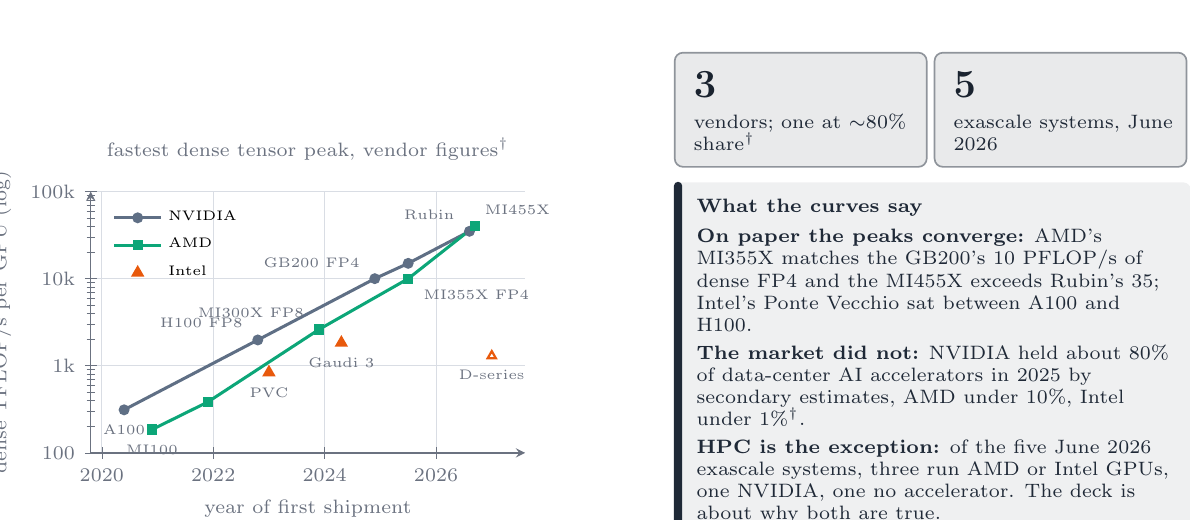
\begin{tikzpicture}
  \useasboundingbox (0,0) rectangle (14.4,5.9);
  \begin{scope}[shift={(0.8,0.5)}]
  \begin{axis}[lecture,width=7.1cm,height=4.9cm,ymode=log,xmin=2019.8,xmax=2027.6,ymin=100,ymax=100000,
      xlabel={year of first shipment},ylabel={dense TFLOP/s per GPU (log)},
      xtick={2020,2022,2024,2026},xticklabel style={/pgf/number format/1000 sep={}},scaled x ticks=false,
      ytick={100,1000,10000,100000},yticklabels={100,1k,10k,100k},
      legend style={at={(0.03,0.97)},anchor=north west,font=\tiny},
      title style={font=\scriptsize,text=muted,at={(0.5,1.02)}},title={fastest dense tensor peak, vendor figures$^\dagger$}]
    \addplot[tok,line width=1.1pt,mark=*,mark size=1.4pt] coordinates {(2020.4,312) (2022.8,1979) (2024.9,10000) (2025.5,15000) (2026.6,35000)};
    \addlegendentry{NVIDIA}
    \addplot[emb,line width=1.1pt,mark=square*,mark size=1.3pt] coordinates {(2020.9,185) (2021.9,383) (2023.9,2615) (2025.5,10000) (2026.7,40260)};
    \addlegendentry{AMD}
    \addplot[attn,line width=1.1pt,mark=triangle*,mark size=1.7pt,only marks] coordinates {(2023.0,839) (2024.3,1835)};
    \addlegendentry{Intel}
    \addplot[attn,mark=triangle,mark size=1.7pt,only marks,line width=0.8pt] coordinates {(2027.0,1300)};
    \node[font=\tiny,text=muted,anchor=north] at (axis cs:2020.4,270) {A100};
    \node[font=\tiny,text=muted,anchor=south east] at (axis cs:2022.7,2100) {H100 FP8};
    \node[font=\tiny,text=muted,anchor=south east] at (axis cs:2024.8,10500) {GB200 FP4};
    \node[font=\tiny,text=muted,anchor=south east] at (axis cs:2026.5,37000) {Rubin};
    \node[font=\tiny,text=muted,anchor=north] at (axis cs:2020.9,160) {MI100};
    \node[font=\tiny,text=muted,anchor=south east] at (axis cs:2023.8,2800) {MI300X FP8};
    \node[font=\tiny,text=muted,anchor=north west] at (axis cs:2025.6,9500) {MI355X FP4};
    \node[font=\tiny,text=muted,anchor=south west] at (axis cs:2026.7,42000) {MI455X};
    \node[font=\tiny,text=muted,anchor=north] at (axis cs:2023.0,720) {PVC};
    \node[font=\tiny,text=muted,anchor=north] at (axis cs:2024.3,1600) {Gaudi 3};
    \node[font=\tiny,text=muted,anchor=north] at (axis cs:2027.0,1150) {D-series};
  \end{axis}
  \end{scope}
  \stat{8.2}{5.6}{3}{vendors; one at ${\sim}$80\% share$^\dagger$}{ink}
  \stat{11.5}{5.6}{5}{exascale systems, June 2026}{ink}
  \bgpanels{8.2}{3.95}{6.0cm}{What the curves say}{%
    \hl{ink}{On paper the peaks converge:} AMD's MI355X matches the
    GB200's 10 PFLOP/s of dense FP4 and the MI455X exceeds Rubin's
    35; Intel's Ponte Vecchio sat between A100 and H100.\\[2pt]
    \hl{ink}{The market did not:} NVIDIA held about 80\% of data-center
    AI accelerators in 2025 by secondary estimates, AMD under 10\%,
    Intel under 1\%$^\dagger$.\\[2pt]
    \hl{ink}{HPC is the exception:} of the five June 2026 exascale
    systems, three run AMD or Intel GPUs, one NVIDIA, one no
    accelerator. The deck is about why both are true.}
\end{tikzpicture}
\end{frame}

% ---------------------------------------------------------------- 3
\begin{frame}{How to compare a platform, and the decade's timeline}
\framesubtitle{A GPU is sold as a package on a board in a rack with a fabric and a software stack; each level is a separate contest.}
\centering
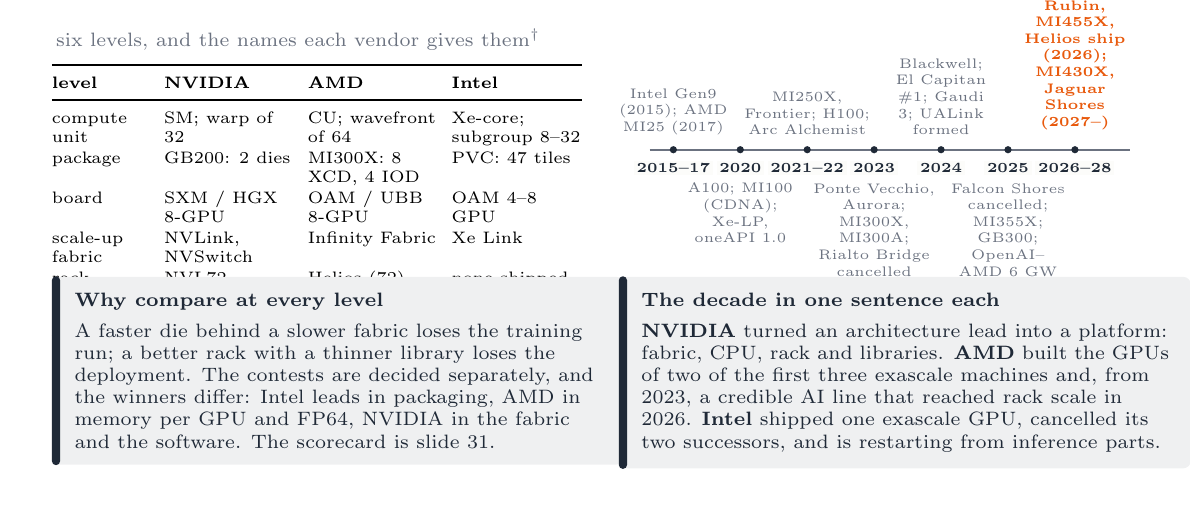
\begin{tikzpicture}
  \useasboundingbox (0,0) rectangle (14.4,5.9);
  \node[lab,anchor=south west] at (0.3,5.55) {six levels, and the names each vendor gives them$^\dagger$};
  \node[anchor=north west,inner sep=0,font=\fontsize{5.8}{6.9}\selectfont] at (0.3,5.45) {%
    \renewcommand{\arraystretch}{1.1}\setlength{\tabcolsep}{2.5pt}%
    \begin{tabular}{@{}>{\raggedright\arraybackslash}p{1.25cm}>{\raggedright\arraybackslash}p{1.65cm}>{\raggedright\arraybackslash}p{1.65cm}>{\raggedright\arraybackslash}p{1.65cm}@{}}
      \toprule
      \textbf{level} & \textbf{NVIDIA} & \textbf{AMD} & \textbf{Intel}\\
      \midrule
      compute unit & SM; warp of 32 & CU; wavefront of 64 & Xe-core; subgroup 8--32\\
      package & GB200: 2 dies & MI300X: 8 XCD, 4 IOD & PVC: 47 tiles\\
      board & SXM / HGX 8-GPU & OAM / UBB 8-GPU & OAM 4--8 GPU\\
      scale-up fabric & NVLink, NVSwitch & Infinity Fabric & Xe Link\\
      rack & NVL72 & Helios (72) & none shipped\\
      software & CUDA & ROCm, HIP & oneAPI, SYCL\\
      \bottomrule
    \end{tabular}};
  \bgpanels{0.3}{2.75}{6.7cm}{Why compare at every level}{%
    A faster die behind a slower fabric loses the training run; a
    better rack with a thinner library loses the deployment. The
    contests are decided separately, and the winners differ: Intel
    leads in packaging, AMD in memory per GPU and FP64, NVIDIA in the
    fabric and the software. The scorecard is slide 31.}
  \draw[muted,line width=0.8pt] (7.9,4.35) -- (14.0,4.35);
  \foreach \x in {8.2,9.05,9.9,10.75,11.6,12.45,13.3}{\fill[ink] (\x,4.35) circle (1.3pt);}
  \foreach \yr/\x in {2015--17/8.2,2020/9.05,2021--22/9.9,2023/10.75,2024/11.6,2025/12.45,2026--28/13.3}{\node[font=\tiny\bfseries,text=ink,fill=paper,inner sep=1pt] at (\x,4.12) {\yr};}
  \node[lab,anchor=south,text width=1.6cm,align=center,font=\tiny] at (8.2,4.48) {Intel Gen9 (2015); AMD MI25 (2017)};
  \node[lab,anchor=north,text width=1.6cm,align=center,font=\tiny] at (9.05,3.98) {A100; MI100 (CDNA); Xe-LP, oneAPI 1.0};
  \node[lab,anchor=south,text width=1.6cm,align=center,font=\tiny] at (9.9,4.48) {MI250X, Frontier; H100; Arc Alchemist};
  \node[lab,anchor=north,text width=1.6cm,align=center,font=\tiny] at (10.75,3.98) {Ponte Vecchio, Aurora; MI300X, MI300A; Rialto Bridge cancelled};
  \node[lab,anchor=south,text width=1.6cm,align=center,font=\tiny] at (11.6,4.48) {Blackwell; El Capitan \#1; Gaudi 3; UALink formed};
  \node[lab,anchor=north,text width=1.6cm,align=center,font=\tiny] at (12.45,3.98) {Falcon Shores cancelled; MI355X; GB300; OpenAI--AMD 6 GW};
  \node[anchor=south,text width=1.6cm,align=center,font=\tiny\bfseries,text=attn] at (13.3,4.48) {Rubin, MI455X, Helios ship (2026); MI430X, Jaguar Shores (2027--)};
  \bgpanels{7.5}{2.75}{6.7cm}{The decade in one sentence each}{%
    \hl{ink}{NVIDIA} turned an architecture lead into a platform:
    fabric, CPU, rack and libraries. \hl{ink}{AMD} built the GPUs of
    two of the first three exascale machines and, from 2023, a
    credible AI line that reached rack scale in 2026. \hl{ink}{Intel} shipped one
    exascale GPU, cancelled its two successors, and is restarting
    from inference parts.}
\end{tikzpicture}
\end{frame}

% ---------------------------------------------------------------- 4
\stage{2}
\begin{frame}{The NVIDIA line as platforms: HGX A100 to Vera Rubin NVL72}
\framesubtitle{Six platforms in six years: the board became a rack, memory grew 7$\times$, the scale-up link 5$\times$, FP64 went up and down.}
\centering
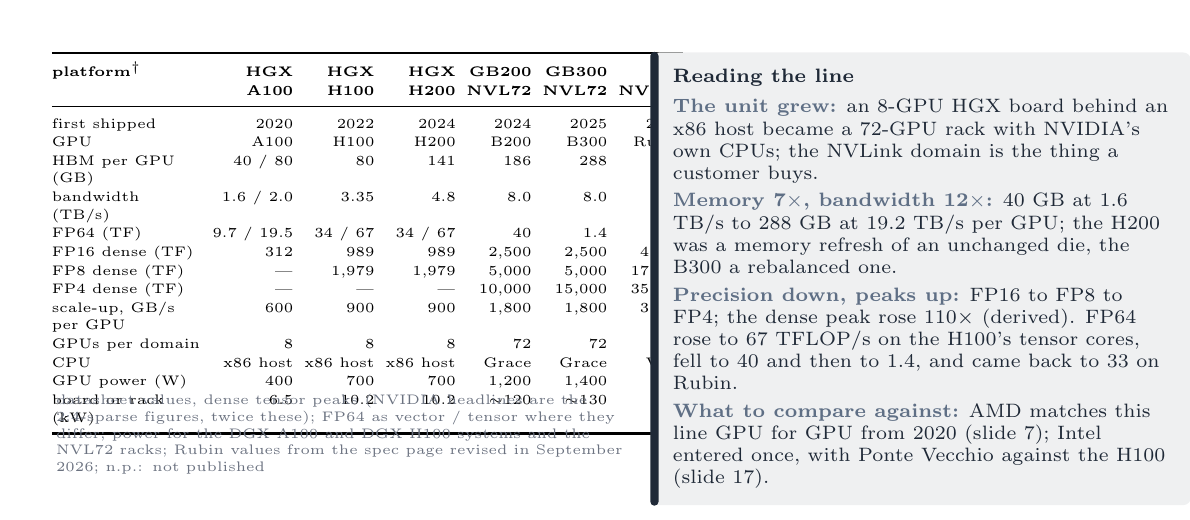
\begin{tikzpicture}
  \useasboundingbox (0,0) rectangle (14.4,5.9);
  \node[anchor=north west,inner sep=0,font=\fontsize{5.4}{6.4}\selectfont] at (0.3,5.6) {%
    \renewcommand{\arraystretch}{1.05}\setlength{\tabcolsep}{2.0pt}%
    \begin{tabular}{@{}>{\raggedright\arraybackslash}p{1.9cm}rrrrrr@{}}
      \toprule
      \textbf{platform}$^\dagger$ & \textbf{HGX} & \textbf{HGX} & \textbf{HGX} & \textbf{GB200} & \textbf{GB300} & \textbf{VR}\\
       & \textbf{A100} & \textbf{H100} & \textbf{H200} & \textbf{NVL72} & \textbf{NVL72} & \textbf{NVL72}\\
      \midrule
      first shipped & 2020 & 2022 & 2024 & 2024 & 2025 & 2026\\
      GPU & A100 & H100 & H200 & B200 & B300 & Rubin\\
      HBM per GPU (GB) & 40 / 80 & 80 & 141 & 186 & 288 & 288\\
      bandwidth (TB/s) & 1.6 / 2.0 & 3.35 & 4.8 & 8.0 & 8.0 & 19.2\\
      FP64 (TF) & 9.7 / 19.5 & 34 / 67 & 34 / 67 & 40 & 1.4 & 33\\
      FP16 dense (TF) & 312 & 989 & 989 & 2{,}500 & 2{,}500 & 4{,}000\\
      FP8 dense (TF) & --- & 1{,}979 & 1{,}979 & 5{,}000 & 5{,}000 & 17{,}500\\
      FP4 dense (TF) & --- & --- & --- & 10{,}000 & 15{,}000 & 35{,}000\\
      scale-up, GB/s per GPU & 600 & 900 & 900 & 1{,}800 & 1{,}800 & 3{,}000\\
      GPUs per domain & 8 & 8 & 8 & 72 & 72 & 72\\
      CPU & x86 host & x86 host & x86 host & Grace & Grace & Vera\\
      GPU power (W) & 400 & 700 & 700 & 1{,}200 & 1{,}400 & n.p.\\
      board or rack (kW) & 6.5 & 10.2 & 10.2 & ${\sim}$120 & ${\sim}$130 & n.p.\\
      \bottomrule
    \end{tabular}};
  \node[lab,font=\tiny,anchor=north west,text width=7.2cm] at (0.3,1.3) {datasheet values, dense tensor peaks (NVIDIA headlines are the 2:4-sparse figures, twice these); FP64 as vector / tensor where they differ; power for the DGX A100 and DGX H100 systems and the NVL72 racks; Rubin values from the spec page revised in September 2026; n.p.: not published};
  \bgpanels{7.9}{5.6}{6.3cm}{Reading the line}{%
    \hl{tok}{The unit grew:} an 8-GPU HGX board behind an x86 host
    became a 72-GPU rack with NVIDIA's own CPUs; the NVLink domain is
    the thing a customer buys.\\[2pt]
    \hl{tok}{Memory 7$\times$, bandwidth 12$\times$:} 40 GB at 1.6
    TB/s to 288 GB at 19.2 TB/s per GPU; the H200 was a memory
    refresh of an unchanged die, the B300 a rebalanced one.\\[2pt]
    \hl{tok}{Precision down, peaks up:} FP16 to FP8 to FP4; the dense
    peak rose 110$\times$ (derived). FP64 rose to 67 TFLOP/s on the
    H100's tensor cores, fell to 40 and then to 1.4, and came back to
    33 on Rubin.\\[2pt]
    \hl{tok}{What to compare against:} AMD matches this line GPU for
    GPU from 2020 (slide 7); Intel entered once, with Ponte Vecchio
    against the H100 (slide 17).}
\end{tikzpicture}
\end{frame}

% ---------------------------------------------------------------- 5
\begin{frame}{Memory per GPU: the contest AMD kept winning on paper}
\framesubtitle{HBM per GPU, 2020--2026: AMD led from the MI250X on and tied in 2025; Ponte Vecchio matched it in 2023.}
\centering
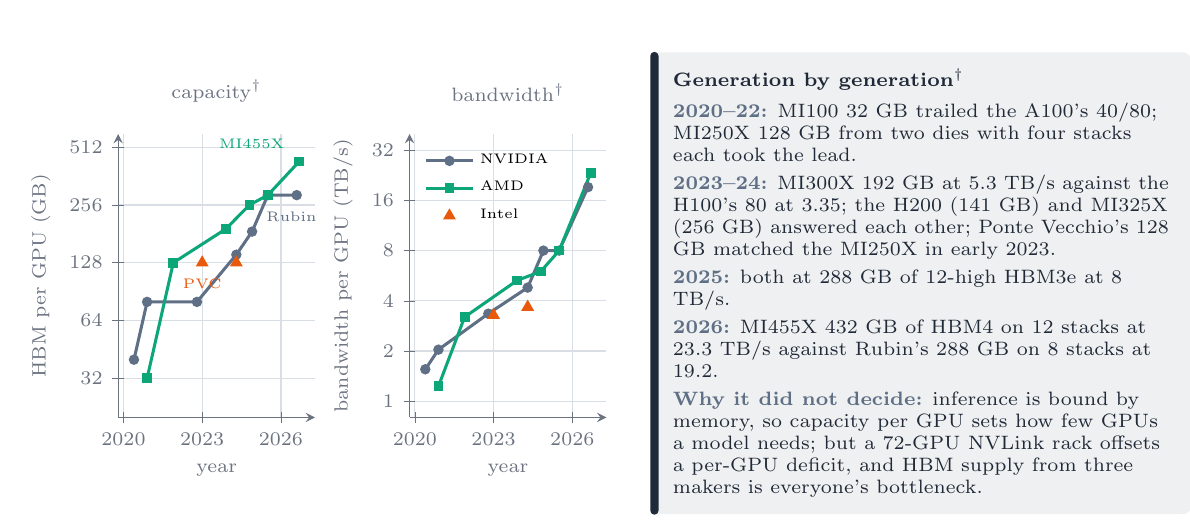
\begin{tikzpicture}
  \useasboundingbox (0,0) rectangle (14.4,5.9);
  \begin{scope}[shift={(1.15,0.95)}]
  \begin{axis}[lecture,scale only axis,width=2.5cm,height=3.6cm,ymode=log,xmin=2019.8,xmax=2027.3,ymin=20,ymax=600,
      xlabel={year},ylabel={HBM per GPU (GB)},
      xtick={2020,2023,2026},xticklabel style={/pgf/number format/1000 sep={}},scaled x ticks=false,
      ytick={32,64,128,256,512},yticklabels={32,64,128,256,512},
      title style={font=\scriptsize,text=muted,at={(0.5,1.02)}},title={capacity$^\dagger$}]
    \addplot[tok,line width=1.1pt,mark=*,mark size=1.3pt] coordinates {(2020.4,40) (2020.9,80) (2022.8,80) (2024.3,141) (2024.9,186) (2025.5,288) (2026.6,288)};
    \addplot[emb,line width=1.1pt,mark=square*,mark size=1.2pt] coordinates {(2020.9,32) (2021.9,128) (2023.9,192) (2024.8,256) (2025.5,288) (2026.7,432)};
    \addplot[attn,line width=1.1pt,mark=triangle*,mark size=1.6pt,only marks] coordinates {(2023.0,128) (2024.3,128)};
    \node[font=\tiny,text=emb,anchor=south east] at (axis cs:2026.5,450) {MI455X};
    \node[font=\tiny,text=tok,anchor=north] at (axis cs:2026.4,265) {Rubin};
    \node[font=\tiny,text=attn,anchor=north] at (axis cs:2023.0,118) {PVC};
  \end{axis}
  \end{scope}
  \begin{scope}[shift={(4.85,0.95)}]
  \begin{axis}[lecture,scale only axis,width=2.5cm,height=3.6cm,ymode=log,xmin=2019.8,xmax=2027.3,ymin=0.8,ymax=40,
      xlabel={year},ylabel={bandwidth per GPU (TB/s)},
      xtick={2020,2023,2026},xticklabel style={/pgf/number format/1000 sep={}},scaled x ticks=false,
      ytick={1,2,4,8,16,32},yticklabels={1,2,4,8,16,32},
      legend style={at={(0.03,0.97)},anchor=north west,font=\tiny},
      title style={font=\scriptsize,text=muted,at={(0.5,1.02)}},title={bandwidth$^\dagger$}]
    \addplot[tok,line width=1.1pt,mark=*,mark size=1.3pt] coordinates {(2020.4,1.555) (2020.9,2.039) (2022.8,3.35) (2024.3,4.8) (2024.9,8) (2025.5,8) (2026.6,19.2)};
    \addlegendentry{NVIDIA}
    \addplot[emb,line width=1.1pt,mark=square*,mark size=1.2pt] coordinates {(2020.9,1.23) (2021.9,3.2) (2023.9,5.3) (2024.8,6.0) (2025.5,8.0) (2026.7,23.3)};
    \addlegendentry{AMD}
    \addplot[attn,line width=1.1pt,mark=triangle*,mark size=1.6pt,only marks] coordinates {(2023.0,3.28) (2024.3,3.67)};
    \addlegendentry{Intel}
  \end{axis}
  \end{scope}
  \bgpanels{7.9}{5.6}{6.3cm}{Generation by generation$^\dagger$}{%
    \hl{tok}{2020--22:} MI100 32 GB trailed the A100's 40/80; MI250X
    128 GB from two dies with four stacks each took the lead.\\[2pt]
    \hl{tok}{2023--24:} MI300X 192 GB at 5.3 TB/s against the H100's
    80 at 3.35; the H200 (141 GB) and MI325X (256 GB) answered each
    other; Ponte Vecchio's 128 GB matched the MI250X in early 2023.\\[2pt]
    \hl{tok}{2025:} both at 288 GB of 12-high HBM3e at 8 TB/s.\\[2pt]
    \hl{tok}{2026:} MI455X 432 GB of HBM4 on 12 stacks at 23.3 TB/s
    against Rubin's 288 GB on 8 stacks at 19.2.\\[2pt]
    \hl{tok}{Why it did not decide:} inference is bound by memory, so
    capacity per GPU sets how few GPUs a model needs; but a 72-GPU
    NVLink rack offsets a per-GPU deficit, and HBM supply from three
    makers is everyone's bottleneck.}
\end{tikzpicture}
\end{frame}

% ---------------------------------------------------------------- 6
\begin{frame}{Compute peaks per GPU: three vendors, FP64 to FP4}
\framesubtitle{Dense vendor peaks; AMD doubled FP64 on matrix cores until CDNA 4; Intel's PVC ran FP64 at full rate.}
\centering
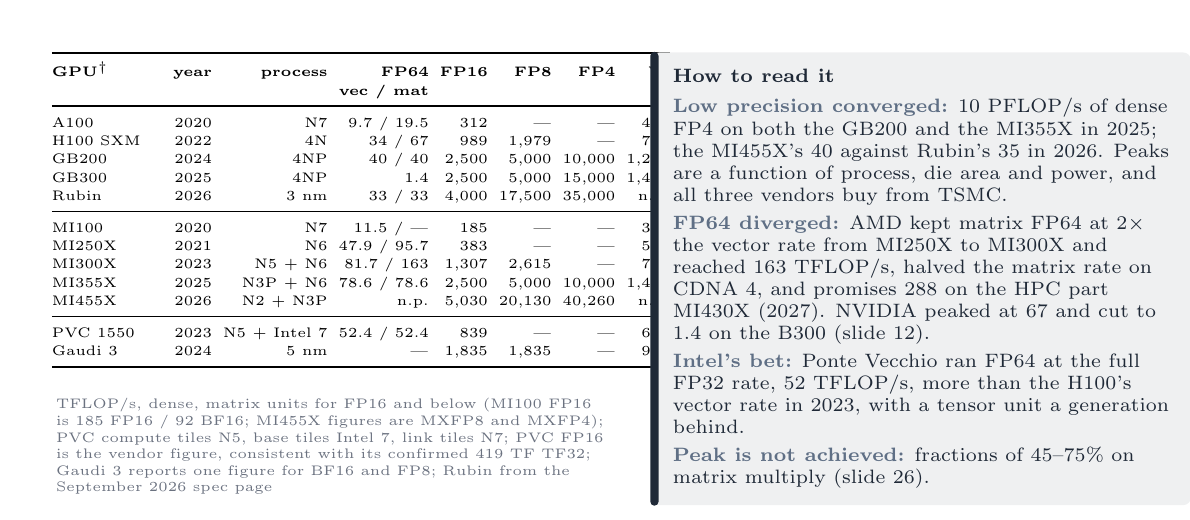
\begin{tikzpicture}
  \useasboundingbox (0,0) rectangle (14.4,5.9);
  \node[anchor=north west,inner sep=0,font=\fontsize{5.4}{6.4}\selectfont] at (0.3,5.6) {%
    \renewcommand{\arraystretch}{1.03}\setlength{\tabcolsep}{2.0pt}%
    \begin{tabular}{@{}>{\raggedright\arraybackslash}p{1.4cm}rrrrrrr@{}}
      \toprule
      \textbf{GPU}$^\dagger$ & \textbf{year} & \textbf{process} & \textbf{FP64} & \textbf{FP16} & \textbf{FP8} & \textbf{FP4} & \textbf{W}\\
       & & & \textbf{vec / mat} & & & & \\
      \midrule
      A100 & 2020 & N7 & 9.7 / 19.5 & 312 & --- & --- & 400\\
      H100 SXM & 2022 & 4N & 34 / 67 & 989 & 1{,}979 & --- & 700\\
      GB200 & 2024 & 4NP & 40 / 40 & 2{,}500 & 5{,}000 & 10{,}000 & 1{,}200\\
      GB300 & 2025 & 4NP & 1.4 & 2{,}500 & 5{,}000 & 15{,}000 & 1{,}400\\
      Rubin & 2026 & 3 nm & 33 / 33 & 4{,}000 & 17{,}500 & 35{,}000 & n.p.\\
      \midrule
      MI100 & 2020 & N7 & 11.5 / --- & 185 & --- & --- & 300\\
      MI250X & 2021 & N6 & 47.9 / 95.7 & 383 & --- & --- & 560\\
      MI300X & 2023 & N5 + N6 & 81.7 / 163 & 1{,}307 & 2{,}615 & --- & 750\\
      MI355X & 2025 & N3P + N6 & 78.6 / 78.6 & 2{,}500 & 5{,}000 & 10{,}000 & 1{,}400\\
      MI455X & 2026 & N2 + N3P & n.p. & 5{,}030 & 20{,}130 & 40{,}260 & n.p.\\
      \midrule
      PVC 1550 & 2023 & N5 + Intel 7 & 52.4 / 52.4 & 839 & --- & --- & 600\\
      Gaudi 3 & 2024 & 5 nm & --- & 1{,}835 & 1{,}835 & --- & 900\\
      \bottomrule
    \end{tabular}};
  \node[lab,font=\tiny,anchor=north west,text width=7.2cm] at (0.3,1.25) {TFLOP/s, dense, matrix units for FP16 and below (MI100 FP16 is 185 FP16 / 92 BF16; MI455X figures are MXFP8 and MXFP4); PVC compute tiles N5, base tiles Intel 7, link tiles N7; PVC FP16 is the vendor figure, consistent with its confirmed 419 TF TF32; Gaudi 3 reports one figure for BF16 and FP8; Rubin from the September 2026 spec page};
  \bgpanels{7.9}{5.6}{6.3cm}{How to read it}{%
    \hl{tok}{Low precision converged:} 10 PFLOP/s of dense FP4 on
    both the GB200 and the MI355X in 2025; the MI455X's 40 against
    Rubin's 35 in 2026. Peaks are a function of process, die area
    and power, and all three vendors buy from TSMC.\\[2pt]
    \hl{tok}{FP64 diverged:} AMD kept matrix FP64 at 2$\times$ the
    vector rate from MI250X to MI300X and reached 163 TFLOP/s, halved
    the matrix rate on CDNA 4, and promises 288 on the HPC part MI430X
    (2027). NVIDIA peaked at 67 and cut to 1.4 on the B300 (slide
    12).\\[2pt]
    \hl{tok}{Intel's bet:} Ponte Vecchio ran FP64 at the full FP32
    rate, 52 TFLOP/s, more than the H100's vector rate in 2023, with
    a tensor unit a generation behind.\\[2pt]
    \hl{tok}{Peak is not achieved:} fractions of 45--75\% on matrix
    multiply (slide 26).}
\end{tikzpicture}
\end{frame}

% ---------------------------------------------------------------- 7
\stage{3}
\begin{frame}{AMD Instinct and CDNA: the compute unit, five generations}
\framesubtitle{A GCN-derived CU with 64-wide wavefronts (32 on CDNA 5) and matrix cores, from one die to a dozen chiplets.}
\centering
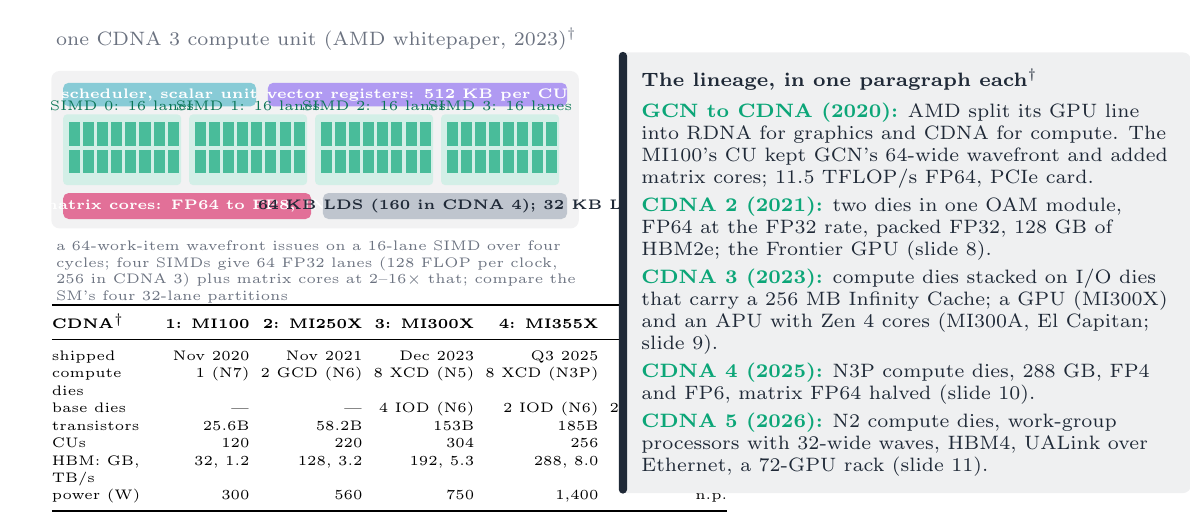
\begin{tikzpicture}
  \useasboundingbox (0,0) rectangle (14.4,5.9);
  \node[lab,anchor=south west] at (0.3,5.55) {one CDNA 3 compute unit (AMD whitepaper, 2023)$^\dagger$};
  \begin{scope}[shift={(0.3,3.35)}]
    \fill[ink!6,rounded corners=3pt] (0,0) rectangle (6.7,2.0);
    \fill[vc!50,rounded corners=2pt] (0.15,1.55) rectangle (2.6,1.85); \node[font=\fontsize{4.5}{5}\selectfont\bfseries,text=white] at (1.375,1.7) {scheduler, scalar unit};
    \fill[posc!55,rounded corners=2pt] (2.75,1.55) rectangle (6.55,1.85); \node[font=\fontsize{4.5}{5}\selectfont\bfseries,text=white] at (4.65,1.7) {vector registers: 512 KB per CU};
    \foreach \q in {0,...,3}{
      \fill[emb!18,rounded corners=1.5pt] (0.15+\q*1.6,0.55) rectangle ++(1.5,0.9);
      \foreach \c in {0,...,7}{\fill[emb!75] (0.22+\q*1.6+\c*0.18,1.05) rectangle ++(0.14,0.3); \fill[emb!75] (0.22+\q*1.6+\c*0.18,0.7) rectangle ++(0.14,0.3);}
      \node[font=\fontsize{4.5}{5}\selectfont,text=emb!70!black,anchor=south] at (0.9+\q*1.6,1.37) {SIMD \q: 16 lanes};}
    \fill[outc!70,rounded corners=2pt] (0.15,0.12) rectangle (3.3,0.45); \node[font=\fontsize{4.5}{5}\selectfont\bfseries,text=white] at (1.725,0.285) {4 matrix cores: FP64 to FP8, INT8};
    \fill[tok!40,rounded corners=2pt] (3.45,0.12) rectangle (6.55,0.45); \node[font=\fontsize{4.5}{5}\selectfont\bfseries,text=ink] at (5.0,0.285) {64 KB LDS (160 in CDNA 4); 32 KB L1};
  \end{scope}
  \node[lab,font=\tiny,anchor=north west,text width=6.7cm] at (0.3,3.25) {a 64-work-item wavefront issues on a 16-lane SIMD over four cycles; four SIMDs give 64 FP32 lanes (128 FLOP per clock, 256 in CDNA 3) plus matrix cores at 2--16$\times$ that; compare the SM's four 32-lane partitions};
  \node[anchor=north west,inner sep=0,font=\fontsize{5.2}{6.2}\selectfont] at (0.3,2.4) {%
    \renewcommand{\arraystretch}{1.02}\setlength{\tabcolsep}{2.0pt}%
    \begin{tabular}{@{}>{\raggedright\arraybackslash}p{1.3cm}rrrrr@{}}
      \toprule
      \textbf{CDNA}$^\dagger$ & \textbf{1: MI100} & \textbf{2: MI250X} & \textbf{3: MI300X} & \textbf{4: MI355X} & \textbf{5: MI455X}\\
      \midrule
      shipped & Nov 2020 & Nov 2021 & Dec 2023 & Q3 2025 & Q3 2026\\
      compute dies & 1 (N7) & 2 GCD (N6) & 8 XCD (N5) & 8 XCD (N3P) & 8 XCD (N2)\\
      base dies & --- & --- & 4 IOD (N6) & 2 IOD (N6) & 2 IOD, 2 FCD\\
      transistors & 25.6B & 58.2B & 153B & 185B & 320B\\
      CUs & 120 & 220 & 304 & 256 & 256 WGP\\
      HBM: GB, TB/s & 32, 1.2 & 128, 3.2 & 192, 5.3 & 288, 8.0 & 432, 23.3\\
      power (W) & 300 & 560 & 750 & 1{,}400 & n.p.\\
      \bottomrule
    \end{tabular}};
  \bgpanels{7.5}{5.6}{6.7cm}{The lineage, in one paragraph each$^\dagger$}{%
    \hl{emb}{GCN to CDNA (2020):} AMD split its GPU line into RDNA for
    graphics and CDNA for compute. The MI100's CU kept GCN's 64-wide
    wavefront and added matrix cores; 11.5 TFLOP/s FP64, PCIe card.\\[2pt]
    \hl{emb}{CDNA 2 (2021):} two dies in one OAM module, FP64 at the
    FP32 rate, packed FP32, 128 GB of HBM2e; the Frontier GPU
    (slide 8).\\[2pt]
    \hl{emb}{CDNA 3 (2023):} compute dies stacked on I/O dies that
    carry a 256 MB Infinity Cache; a GPU (MI300X) and an APU with
    Zen 4 cores (MI300A, El Capitan; slide 9).\\[2pt]
    \hl{emb}{CDNA 4 (2025):} N3P compute dies, 288 GB, FP4 and FP6,
    matrix FP64 halved (slide 10).\\[2pt]
    \hl{emb}{CDNA 5 (2026):} N2 compute dies, work-group processors
    with 32-wide waves, HBM4, UALink over Ethernet, a 72-GPU rack
    (slide 11).}
\end{tikzpicture}
\end{frame}

% ---------------------------------------------------------------- 8
\begin{frame}{MI250X and Frontier: two dies per module and the first exaflop}
\framesubtitle{Each MI250X holds two compute dies that software sees as two GPUs; 37,632 of them made Frontier (2022).}
\centering
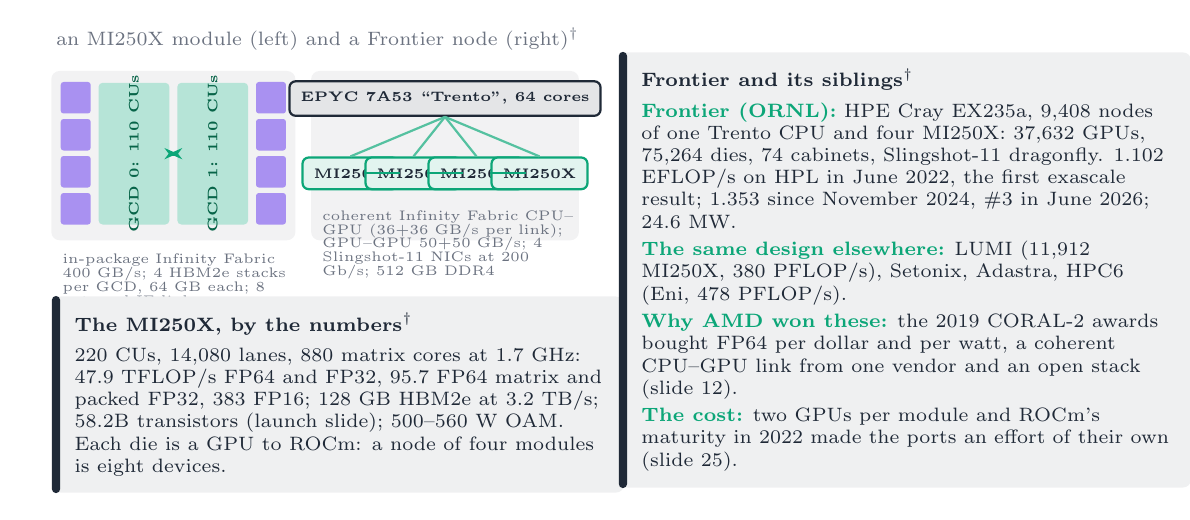
\begin{tikzpicture}
  \useasboundingbox (0,0) rectangle (14.4,5.9);
  \node[lab,anchor=south west] at (0.3,5.55) {an MI250X module (left) and a Frontier node (right)$^\dagger$};
  \begin{scope}[shift={(0.3,3.2)}]
    \fill[ink!6,rounded corners=3pt] (0,0) rectangle (3.1,2.15);
    \foreach \s in {0,...,3}{\fill[posc!60,rounded corners=1pt] (0.12,0.2+\s*0.47) rectangle ++(0.38,0.4); \fill[posc!60,rounded corners=1pt] (2.6,0.2+\s*0.47) rectangle ++(0.38,0.4);}
    \fill[emb!30,rounded corners=1.5pt] (0.6,0.2) rectangle (1.5,2.0); \fill[emb!30,rounded corners=1.5pt] (1.6,0.2) rectangle (2.5,2.0);
    \node[font=\fontsize{4.5}{5}\selectfont\bfseries,text=emb!60!black,rotate=90] at (1.05,1.1) {GCD 0: 110 CUs}; \node[font=\fontsize{4.5}{5}\selectfont\bfseries,text=emb!60!black,rotate=90] at (2.05,1.1) {GCD 1: 110 CUs};
    \draw[emb,line width=1.5pt,<->] (1.5,1.1) -- (1.6,1.1);
    \node[font=\fontsize{4.5}{5}\selectfont,text=muted,anchor=north west,text width=3.0cm] at (0.02,-0.05) {in-package Infinity Fabric 400 GB/s; 4 HBM2e stacks per GCD, 64 GB each; 8 external IF links};
  \end{scope}
  \begin{scope}[shift={(3.6,3.2)}]
    \fill[ink!6,rounded corners=3pt] (0,0) rectangle (3.4,2.15);
    \node[comp=ink,minimum width=1.6cm,minimum height=0.42cm,font=\fontsize{4.5}{5}\selectfont\bfseries,text=ink] (cpu) at (1.7,1.8) {EPYC 7A53 ``Trento'', 64 cores};
    \foreach \g in {0,...,3}{\node[comp=emb,minimum width=0.7cm,minimum height=0.4cm,font=\fontsize{4.5}{5}\selectfont\bfseries,text=ink] (g\g) at (0.5+\g*0.8,0.85) {MI250X};
      \draw[emb!70,line width=0.8pt] (cpu.south) -- (g\g.north);}
    \draw[emb,line width=0.8pt] (g0) -- (g1); \draw[emb,line width=0.8pt] (g1) -- (g2); \draw[emb,line width=0.8pt] (g2) -- (g3);
    \node[font=\fontsize{4.5}{5}\selectfont,text=muted,anchor=north west,text width=3.3cm] at (0.02,0.5) {coherent Infinity Fabric CPU--GPU (36$+$36 GB/s per link); GPU--GPU 50$+$50 GB/s; 4 Slingshot-11 NICs at 200 Gb/s; 512 GB DDR4};
  \end{scope}
  \bgpanels{0.3}{2.5}{6.7cm}{The MI250X, by the numbers$^\dagger$}{%
    220 CUs, 14{,}080 lanes, 880 matrix cores at 1.7 GHz: 47.9
    TFLOP/s FP64 and FP32, 95.7 FP64 matrix and packed FP32, 383
    FP16; 128 GB HBM2e at 3.2 TB/s; 58.2B transistors (launch slide);
    500--560 W OAM. Each die is a GPU to ROCm: a node of four modules
    is eight devices.}
  \bgpanels{7.5}{5.6}{6.7cm}{Frontier and its siblings$^\dagger$}{%
    \hl{emb}{Frontier (ORNL):} HPE Cray EX235a, 9{,}408 nodes of one
    Trento CPU and four MI250X: 37{,}632 GPUs, 75{,}264 dies, 74
    cabinets, Slingshot-11 dragonfly. 1.102 EFLOP/s on HPL in June
    2022, the first exascale result; 1.353 since November 2024, \#3
    in June 2026; 24.6 MW.\\[2pt]
    \hl{emb}{The same design elsewhere:} LUMI (11{,}912 MI250X, 380
    PFLOP/s), Setonix, Adastra, HPC6 (Eni, 478 PFLOP/s).\\[2pt]
    \hl{emb}{Why AMD won these:} the 2019 CORAL-2 awards bought FP64
    per dollar and per watt, a coherent CPU--GPU link from one vendor
    and an open stack (slide 12).\\[2pt]
    \hl{emb}{The cost:} two GPUs per module and ROCm's maturity in
    2022 made the ports an effort of their own (slide 25).}
\end{tikzpicture}
\end{frame}

% ---------------------------------------------------------------- 9
\begin{frame}{MI300X and MI300A: 3D chiplets and the exascale APU}
\framesubtitle{Eight compute dies stacked on four I/O dies with a 256 MB cache; with CPU cores it became El Capitan.}
\centering
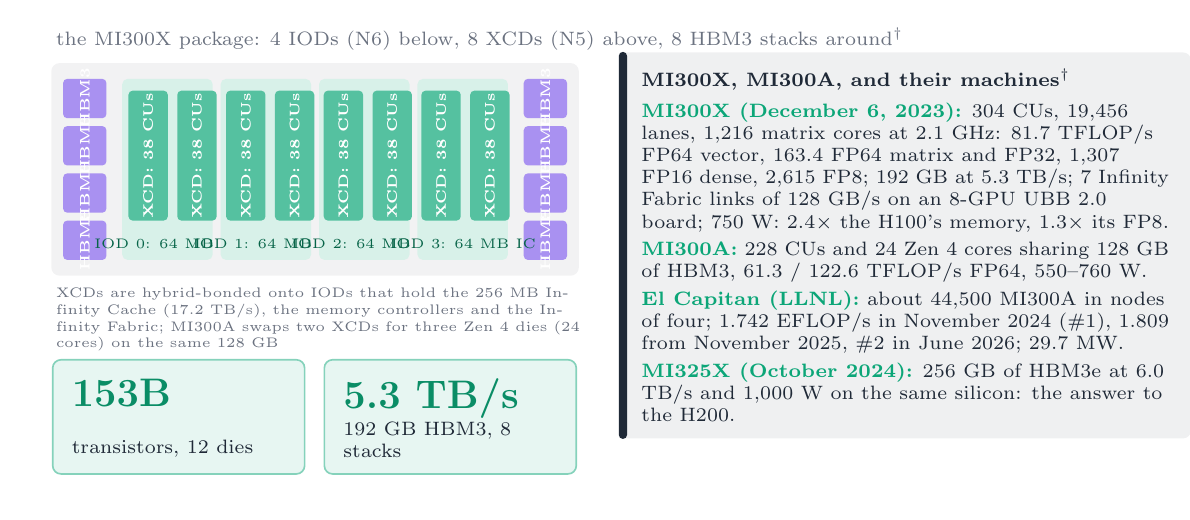
\begin{tikzpicture}
  \useasboundingbox (0,0) rectangle (14.4,5.9);
  \node[lab,anchor=south west] at (0.3,5.55) {the MI300X package: 4 IODs (N6) below, 8 XCDs (N5) above, 8 HBM3 stacks around$^\dagger$};
  \begin{scope}[shift={(0.3,2.75)}]
    \fill[ink!6,rounded corners=3pt] (0,0) rectangle (6.7,2.7);
    \foreach \s in {0,...,3}{\fill[posc!60,rounded corners=1.5pt] (0.15,0.2+\s*0.6) rectangle ++(0.55,0.5); \node[font=\fontsize{4.5}{5}\selectfont\bfseries,text=white,rotate=90] at (0.425,0.45+\s*0.6) {HBM3};
      \fill[posc!60,rounded corners=1.5pt] (6.0,0.2+\s*0.6) rectangle ++(0.55,0.5); \node[font=\fontsize{4.5}{5}\selectfont\bfseries,text=white,rotate=90] at (6.275,0.45+\s*0.6) {HBM3};}
    \foreach \i in {0,...,3}{\fill[emb!16,rounded corners=2pt] (0.9+\i*1.25,0.2) rectangle ++(1.15,2.3);
      \node[font=\fontsize{4.5}{5}\selectfont,text=emb!60!black] at (1.475+\i*1.25,0.4) {IOD \i: 64 MB IC};}
    \foreach \i in {0,...,7}{\fill[emb!70,rounded corners=1.5pt] (0.98+\i*0.62,0.7) rectangle ++(0.5,1.65); \node[font=\fontsize{4.5}{5}\selectfont\bfseries,text=white,rotate=90] at (1.23+\i*0.62,1.52) {XCD: 38 CUs};}
  \end{scope}
  \node[lab,font=\tiny,anchor=north west,text width=6.7cm] at (0.3,2.65) {XCDs are hybrid-bonded onto IODs that hold the 256 MB Infinity Cache (17.2 TB/s), the memory controllers and the Infinity Fabric; MI300A swaps two XCDs for three Zen 4 dies (24 cores) on the same 128 GB};
  \stat{0.3}{1.7}{153B}{transistors, 12 dies}{emb}
  \stat{3.75}{1.7}{5.3 TB/s}{192 GB HBM3, 8 stacks}{emb}
  \bgpanels{7.5}{5.6}{6.7cm}{MI300X, MI300A, and their machines$^\dagger$}{%
    \hl{emb}{MI300X (December 6, 2023):} 304 CUs, 19{,}456 lanes,
    1{,}216 matrix cores at 2.1 GHz: 81.7 TFLOP/s FP64 vector, 163.4
    FP64 matrix and FP32, 1{,}307 FP16 dense, 2{,}615 FP8; 192 GB at
    5.3 TB/s; 7 Infinity Fabric links of 128 GB/s on an 8-GPU UBB 2.0
    board; 750 W: 2.4$\times$ the H100's memory, 1.3$\times$ its FP8.\\[2pt]
    \hl{emb}{MI300A:} 228 CUs and 24 Zen 4 cores sharing 128 GB of
    HBM3, 61.3 / 122.6 TFLOP/s FP64, 550--760 W.\\[2pt]
    \hl{emb}{El Capitan (LLNL):} about 44{,}500 MI300A in nodes of
    four; 1.742 EFLOP/s in November 2024 (\#1), 1.809 from November
    2025, \#2 in June 2026; 29.7 MW.\\[2pt]
    \hl{emb}{MI325X (October 2024):} 256 GB of HBM3e at 6.0 TB/s and
    1{,}000 W on the same silicon: the answer to the H200.}
\end{tikzpicture}
\end{frame}

% ---------------------------------------------------------------- 10
\begin{frame}{CDNA 4: MI355X, 288 GB and FP4, matrix FP64 halved}
\framesubtitle{The same recipe as Blackwell Ultra one quarter later: more HBM, 4-bit formats, less double precision, 1,400 W.}
\centering
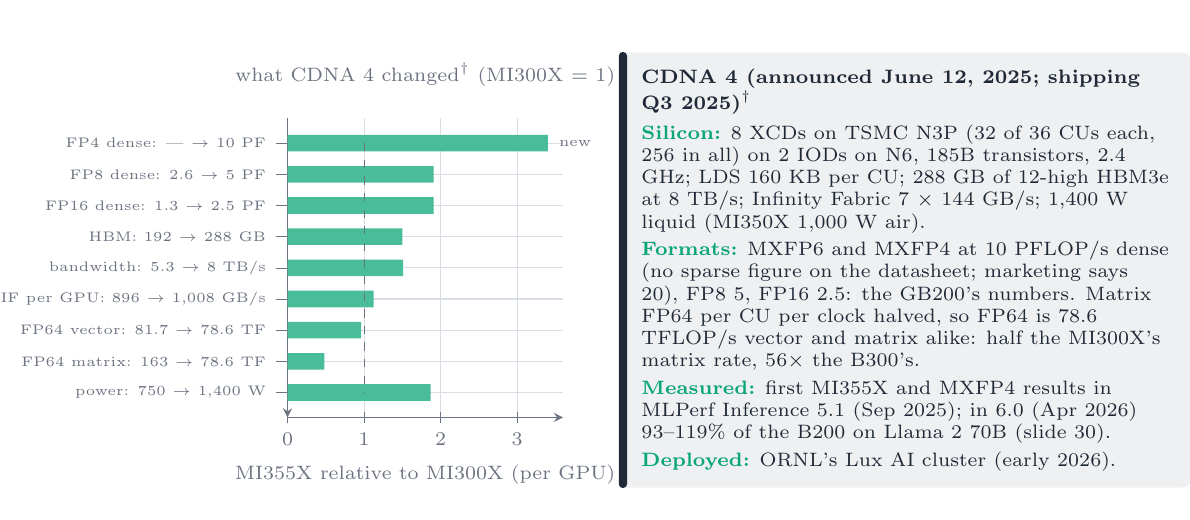
\begin{tikzpicture}
  \useasboundingbox (0,0) rectangle (14.4,5.9);
  \begin{scope}[shift={(3.3,0.95)}]
  \begin{axis}[lecture,scale only axis,width=3.5cm,height=3.8cm,xbar,bar width=6pt,xmin=0,xmax=3.6,enlarge y limits=0.1,
      symbolic y coords={{FP4 dense: --- $\to$ 10 PF},{FP8 dense: 2.6 $\to$ 5 PF},{FP16 dense: 1.3 $\to$ 2.5 PF},{HBM: 192 $\to$ 288 GB},{bandwidth: 5.3 $\to$ 8 TB/s},{IF per GPU: 896 $\to$ 1{,}008 GB/s},{FP64 vector: 81.7 $\to$ 78.6 TF},{FP64 matrix: 163 $\to$ 78.6 TF},{power: 750 $\to$ 1{,}400 W}},
      ytick=data,y dir=reverse,yticklabel style={font=\tiny},xlabel={MI355X relative to MI300X (per GPU)},
      xtick={0,1,2,3},
      title style={font=\scriptsize,text=muted,at={(0.5,1.02)}},title={what CDNA 4 changed$^\dagger$ (MI300X $=$ 1)}]
    \addplot[fill=emb!75,draw=none] coordinates {(3.4,{FP4 dense: --- $\to$ 10 PF}) (1.91,{FP8 dense: 2.6 $\to$ 5 PF}) (1.91,{FP16 dense: 1.3 $\to$ 2.5 PF}) (1.5,{HBM: 192 $\to$ 288 GB}) (1.51,{bandwidth: 5.3 $\to$ 8 TB/s}) (1.125,{IF per GPU: 896 $\to$ 1{,}008 GB/s}) (0.96,{FP64 vector: 81.7 $\to$ 78.6 TF}) (0.48,{FP64 matrix: 163 $\to$ 78.6 TF}) (1.87,{power: 750 $\to$ 1{,}400 W})};
    \draw[muted,dashed] (axis cs:1,{FP4 dense: --- $\to$ 10 PF}) -- (axis cs:1,{power: 750 $\to$ 1{,}400 W});
    \node[font=\tiny,text=muted,anchor=west] at (axis cs:3.42,{FP4 dense: --- $\to$ 10 PF}) {new};
  \end{axis}
  \end{scope}
  \bgpanels{7.5}{5.6}{6.7cm}{CDNA 4 (announced June 12, 2025; shipping Q3 2025)$^\dagger$}{%
    \hl{emb}{Silicon:} 8 XCDs on TSMC N3P (32 of 36 CUs each, 256 in
    all) on 2 IODs on N6, 185B transistors, 2.4 GHz; LDS 160 KB per
    CU; 288 GB of 12-high HBM3e at 8 TB/s; Infinity Fabric 7 $\times$
    144 GB/s; 1{,}400 W liquid (MI350X 1{,}000 W air).\\[2pt]
    \hl{emb}{Formats:} MXFP6 and MXFP4 at 10 PFLOP/s dense (no sparse
    figure on the datasheet; marketing says 20), FP8 5, FP16 2.5:
    the GB200's numbers.
    Matrix FP64 per CU per clock halved, so FP64 is 78.6 TFLOP/s
    vector and matrix alike: half the MI300X's matrix rate, 56$\times$
    the B300's.\\[2pt]
    \hl{emb}{Measured:} first MI355X and MXFP4 results in MLPerf
    Inference 5.1 (Sep 2025); in 6.0 (Apr 2026) 93--119\% of the
    B200 on Llama 2 70B (slide 30).\\[2pt]
    \hl{emb}{Deployed:} ORNL's Lux AI cluster (early 2026).}
\end{tikzpicture}
\end{frame}

% ---------------------------------------------------------------- 11
\begin{frame}{MI400, MI455X and Helios: AMD's rack (2026)}
\framesubtitle{CDNA 5 on TSMC N2, 432 GB of HBM4, UALink over Ethernet, 72 GPUs per rack; shipping from Q3 2026.}
\centering
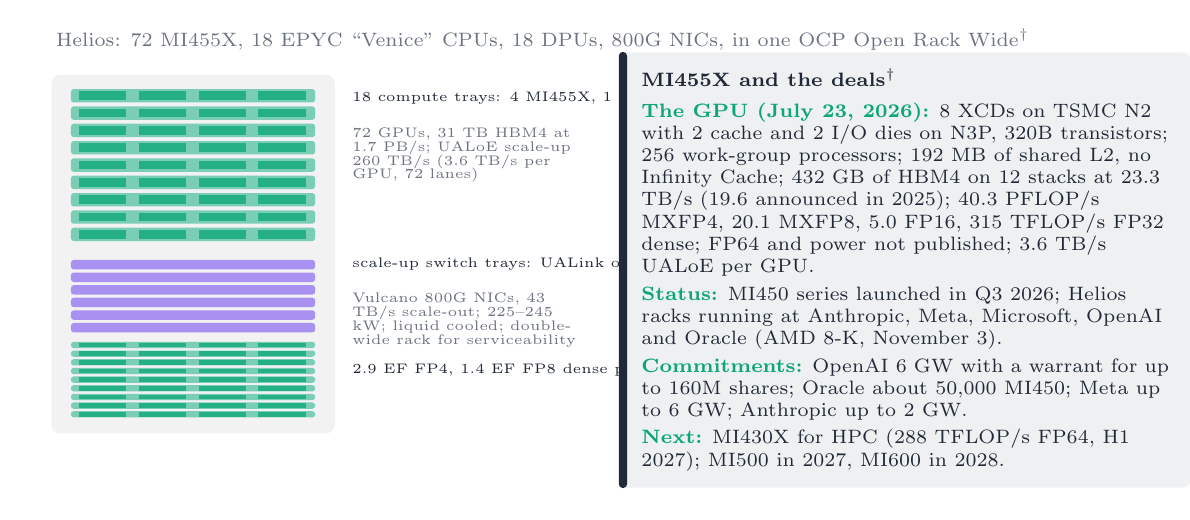
\begin{tikzpicture}
  \useasboundingbox (0,0) rectangle (14.4,5.9);
  \node[lab,anchor=south west] at (0.3,5.55) {Helios: 72 MI455X, 18 EPYC ``Venice'' CPUs, 18 DPUs, 800G NICs, in one OCP Open Rack Wide$^\dagger$};
  \begin{scope}[shift={(0.3,0.75)}]
    \fill[ink!6,rounded corners=3pt] (0,0) rectangle (3.6,4.55);
    \foreach \t in {0,...,8}{\fill[emb!55,rounded corners=1pt] (0.25,4.2-\t*0.22) rectangle (3.35,4.37-\t*0.22);
      \foreach \g in {0,...,3}{\fill[emb!90] (0.35+\g*0.76,4.23-\t*0.22) rectangle ++(0.6,0.11);}}
    \foreach \t in {0,...,5}{\fill[posc!60,rounded corners=1pt] (0.25,2.08-\t*0.16) rectangle (3.35,2.2-\t*0.16);}
    \foreach \t in {0,...,8}{\fill[emb!55,rounded corners=1pt] (0.25,1.08-\t*0.11) rectangle (3.35,1.16-\t*0.11);
      \foreach \g in {0,...,3}{\fill[emb!90] (0.35+\g*0.76,1.09-\t*0.11) rectangle ++(0.6,0.06);}}
    \node[font=\fontsize{4.5}{5}\selectfont,text=ink,anchor=west] at (3.7,4.25) {18 compute trays: 4 MI455X, 1 Venice, 1 Salina DPU each};
    \node[font=\fontsize{4.5}{5}\selectfont,text=muted,anchor=north west,text width=3.0cm] at (3.7,4.0) {72 GPUs, 31 TB HBM4 at 1.7 PB/s; UALoE scale-up 260 TB/s (3.6 TB/s per GPU, 72 lanes)};
    \node[font=\fontsize{4.5}{5}\selectfont,text=ink,anchor=west] at (3.7,2.15) {scale-up switch trays: UALink over Ethernet};
    \node[font=\fontsize{4.5}{5}\selectfont,text=muted,anchor=north west,text width=3.0cm] at (3.7,1.9) {Vulcano 800G NICs, 43 TB/s scale-out; 225--245 kW; liquid cooled; double-wide rack for serviceability};
    \node[font=\fontsize{4.5}{5}\selectfont,text=ink,anchor=west] at (3.7,0.8) {2.9 EF FP4, 1.4 EF FP8 dense per rack};
  \end{scope}
  \bgpanels{7.5}{5.6}{6.7cm}{MI455X and the deals$^\dagger$}{%
    \hl{emb}{The GPU (July 23, 2026):} 8 XCDs on TSMC N2 with 2 cache
    and 2 I/O dies on N3P, 320B transistors; 256 work-group
    processors; 192 MB of shared L2, no Infinity Cache; 432 GB of
    HBM4 on 12 stacks at 23.3 TB/s (19.6 announced in 2025); 40.3
    PFLOP/s MXFP4, 20.1 MXFP8, 5.0 FP16, 315 TFLOP/s FP32 dense; FP64
    and power not published; 3.6 TB/s UALoE per GPU.\\[2pt]
    \hl{emb}{Status:} MI450 series launched in Q3 2026; Helios racks
    running at Anthropic, Meta, Microsoft, OpenAI and Oracle (AMD
    8-K, November 3).\\[2pt]
    \hl{emb}{Commitments:} OpenAI 6 GW with a warrant for up to 160M
    shares; Oracle about 50{,}000 MI450; Meta up to 6 GW; Anthropic
    up to 2 GW.\\[2pt]
    \hl{emb}{Next:} MI430X for HPC (288 TFLOP/s FP64, H1 2027); MI500
    in 2027, MI600 in 2028.}
\end{tikzpicture}
\end{frame}

% ---------------------------------------------------------------- 12
\begin{frame}{FP64 across the three vendors: who still builds for HPC}
\framesubtitle{AMD kept doubling it, NVIDIA cut it, Intel ran it at full rate once; three of five exascale machines are AMD or Intel.}
\centering
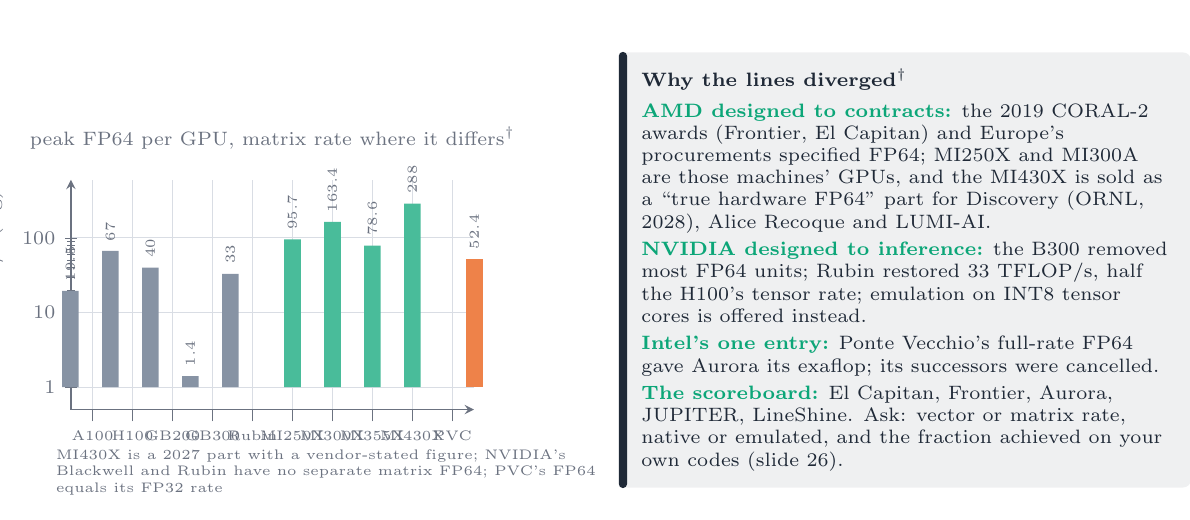
\begin{tikzpicture}
  \useasboundingbox (0,0) rectangle (14.4,5.9);
  \begin{scope}[shift={(0.55,1.05)}]
  \begin{axis}[lecture,width=6.7cm,height=4.5cm,ybar,bar width=6pt,ymode=log,ymin=0.5,ymax=600,enlarge x limits=0.06,
      symbolic x coords={A100,H100,GB200,GB300,Rubin,MI250X,MI300X,MI355X,MI430X,PVC},xtick={A100,H100,GB200,GB300,Rubin,MI250X,MI300X,MI355X,MI430X,PVC},xticklabel style={font=\fontsize{4.3}{5}\selectfont},
      ylabel={FP64 TFLOP/s (log)},ytick={1,10,100},yticklabels={1,10,100},
      nodes near coords,nodes near coords style={font=\tiny,text=muted,rotate=90,anchor=west},point meta=rawy,
      title style={font=\scriptsize,text=muted,at={(0.5,1.02)}},title={peak FP64 per GPU, matrix rate where it differs$^\dagger$}]
    \addplot[fill=tok!75,draw=none] coordinates {(A100,19.5) (H100,67) (GB200,40) (GB300,1.4) (Rubin,33)};
    \addplot[fill=emb!75,draw=none] coordinates {(MI250X,95.7) (MI300X,163.4) (MI355X,78.6) (MI430X,288)};
    \addplot[fill=attn!75,draw=none] coordinates {(PVC,52.4)};
  \end{axis}
  \end{scope}
  \node[lab,font=\tiny,anchor=north west,text width=7.0cm] at (0.3,0.6) {MI430X is a 2027 part with a vendor-stated figure; NVIDIA's Blackwell and Rubin have no separate matrix FP64; PVC's FP64 equals its FP32 rate};
  \bgpanels{7.5}{5.6}{6.7cm}{Why the lines diverged$^\dagger$}{%
    \hl{emb}{AMD designed to contracts:} the 2019 CORAL-2 awards
    (Frontier, El Capitan) and Europe's procurements specified FP64;
    MI250X and MI300A are those machines' GPUs, and the MI430X is
    sold as a ``true hardware FP64'' part for Discovery (ORNL, 2028),
    Alice Recoque and LUMI-AI.\\[2pt]
    \hl{emb}{NVIDIA designed to inference:} the B300 removed most
    FP64 units; Rubin restored 33 TFLOP/s, half the H100's tensor
    rate; emulation on INT8 tensor cores is offered instead.\\[2pt]
    \hl{emb}{Intel's one entry:} Ponte Vecchio's full-rate FP64 gave
    Aurora its exaflop; its successors were cancelled.\\[2pt]
    \hl{emb}{The scoreboard:} El Capitan, Frontier, Aurora, JUPITER,
    LineShine. Ask: vector or matrix rate, native or emulated, and
    the fraction achieved on your own codes (slide 26).}
\end{tikzpicture}
\end{frame}

% ---------------------------------------------------------------- 13
\stage{4}
\begin{frame}{Intel's integrated GPUs: Gen9 to Gen12, the EU and the slice}
\framesubtitle{For a decade Intel's GPU shipped inside every laptop CPU; its EU and slice are what Xe grew from.}
\centering
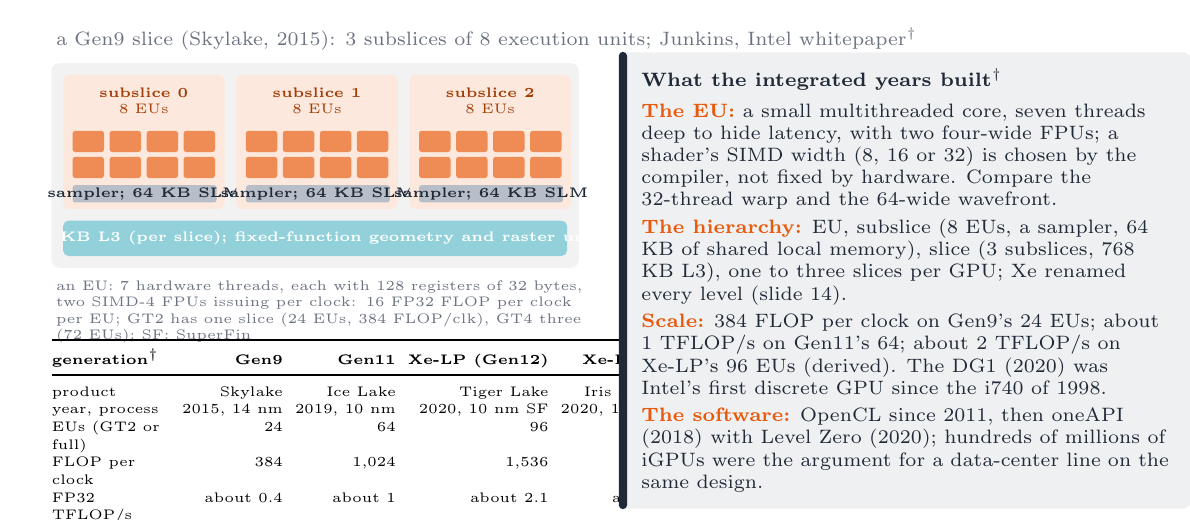
\begin{tikzpicture}
  \useasboundingbox (0,0) rectangle (14.4,5.9);
  \node[lab,anchor=south west] at (0.3,5.55) {a Gen9 slice (Skylake, 2015): 3 subslices of 8 execution units; Junkins, Intel whitepaper$^\dagger$};
  \begin{scope}[shift={(0.3,2.85)}]
    \fill[ink!6,rounded corners=3pt] (0,0) rectangle (6.7,2.6);
    \foreach \s in {0,1,2}{
      \begin{scope}[shift={(0.15+\s*2.2,0.75)}]
        \fill[attn!14,rounded corners=2pt] (0,0) rectangle (2.05,1.7);
        \node[font=\fontsize{4.5}{5}\selectfont\bfseries,text=attn!70!black,anchor=north] at (1.025,1.66) {subslice \s};
        \foreach \r in {0,1}{\foreach \c in {0,...,3}{\fill[attn!70,rounded corners=1pt] (0.12+\c*0.47,0.72-\r*0.33) rectangle ++(0.4,0.27);}}
        \node[font=\fontsize{4.5}{5}\selectfont,text=attn!70!black,anchor=south] at (1.025,1.08) {8 EUs};
        \fill[tok!45,rounded corners=1pt] (0.12,0.08) rectangle (1.95,0.3); \node[font=\fontsize{4.5}{5}\selectfont\bfseries,text=ink] at (1.035,0.19) {sampler; 64 KB SLM};
      \end{scope}}
    \fill[vc!45,rounded corners=2pt] (0.15,0.15) rectangle (6.55,0.6); \node[font=\tiny\bfseries,text=white] at (3.35,0.375) {768 KB L3 (per slice); fixed-function geometry and raster units};
  \end{scope}
  \node[lab,font=\tiny,anchor=north west,text width=6.7cm] at (0.3,2.75) {an EU: 7 hardware threads, each with 128 registers of 32 bytes, two SIMD-4 FPUs issuing per clock: 16 FP32 FLOP per clock per EU; GT2 has one slice (24 EUs, 384 FLOP/clk), GT4 three (72 EUs); SF: SuperFin};
  \node[anchor=north west,inner sep=0,font=\fontsize{5.4}{6.4}\selectfont] at (0.3,1.95) {%
    \renewcommand{\arraystretch}{1.0}\setlength{\tabcolsep}{2.2pt}%
    \begin{tabular}{@{}>{\raggedright\arraybackslash}p{1.5cm}rrrr@{}}
      \toprule
      \textbf{generation}$^\dagger$ & \textbf{Gen9} & \textbf{Gen11} & \textbf{Xe-LP (Gen12)} & \textbf{Xe-LP DG1}\\
      \midrule
      product & Skylake & Ice Lake & Tiger Lake & Iris Xe MAX\\
      year, process & 2015, 14 nm & 2019, 10 nm & 2020, 10 nm SF & 2020, 10 nm SF\\
      EUs (GT2 or full) & 24 & 64 & 96 & 96\\
      FLOP per clock & 384 & 1{,}024 & 1{,}536 & 1{,}536\\
      FP32 TFLOP/s & about 0.4 & about 1 & about 2.1 & about 2.5\\
      \bottomrule
    \end{tabular}};
  \bgpanels{7.5}{5.6}{6.7cm}{What the integrated years built$^\dagger$}{%
    \hl{attn}{The EU:} a small multithreaded core, seven threads deep
    to hide latency, with two four-wide FPUs; a shader's SIMD width
    (8, 16 or 32) is chosen by the compiler, not fixed by hardware.
    Compare the 32-thread warp and the 64-wide wavefront.\\[2pt]
    \hl{attn}{The hierarchy:} EU, subslice (8 EUs, a sampler, 64 KB
    of shared local memory), slice (3 subslices, 768 KB L3), one to
    three slices per GPU; Xe renamed every level (slide 14).\\[2pt]
    \hl{attn}{Scale:} 384 FLOP per clock on Gen9's 24 EUs; about 1
    TFLOP/s on Gen11's 64; about 2 TFLOP/s on Xe-LP's 96 EUs
    (derived). The DG1 (2020) was Intel's first discrete GPU since
    the i740 of 1998.\\[2pt]
    \hl{attn}{The software:} OpenCL since 2011, then oneAPI (2018)
    with Level Zero (2020); hundreds of millions of iGPUs were the
    argument for a data-center line on the same design.}
\end{tikzpicture}
\end{frame}

% ---------------------------------------------------------------- 14
\begin{frame}{From EU to Xe-core: the Xe hierarchy against SM and CU}
\framesubtitle{Xe (2020) renamed the units, doubled the vector width for HPC and added the XMX matrix engine.}
\centering
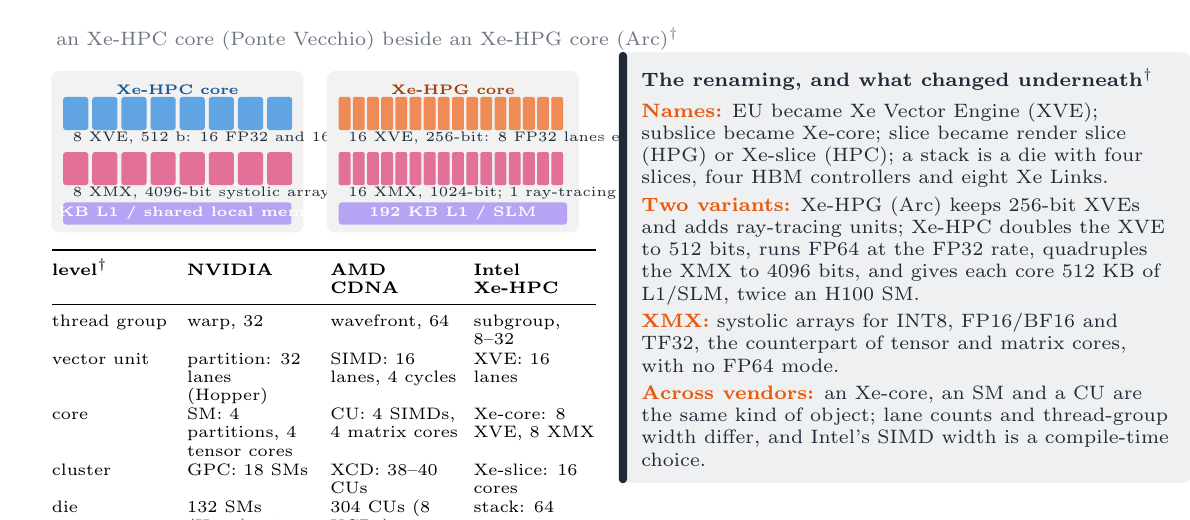
\begin{tikzpicture}
  \useasboundingbox (0,0) rectangle (14.4,5.9);
  \node[lab,anchor=south west] at (0.3,5.55) {an Xe-HPC core (Ponte Vecchio) beside an Xe-HPG core (Arc)$^\dagger$};
  \begin{scope}[shift={(0.3,3.3)}]
    \fill[ink!6,rounded corners=3pt] (0,0) rectangle (3.2,2.05);
    \node[font=\fontsize{4.5}{5}\selectfont\bfseries,text=mlp!70!black,anchor=north] at (1.6,2.0) {Xe-HPC core};
    \foreach \c in {0,...,7}{\fill[mlp!70,rounded corners=1pt] (0.15+\c*0.37,1.3) rectangle ++(0.32,0.42);}
    \node[font=\fontsize{4.5}{5}\selectfont,text=mlp!70!black,anchor=south] at (1.6,1.74) {};
    \node[font=\fontsize{4.5}{5}\selectfont,text=ink,anchor=west] at (0.15,1.2) {8 XVE, 512 b: 16 FP32 and 16 FP64 FMA/clk each};
    \foreach \c in {0,...,7}{\fill[outc!70,rounded corners=1pt] (0.15+\c*0.37,0.6) rectangle ++(0.32,0.42);}
    \node[font=\fontsize{4.5}{5}\selectfont,text=ink,anchor=west] at (0.15,0.5) {8 XMX, 4096-bit systolic arrays};
    \fill[posc!50,rounded corners=1pt] (0.15,0.1) rectangle (3.05,0.38); \node[font=\fontsize{4.5}{5}\selectfont\bfseries,text=white] at (1.6,0.24) {512 KB L1 / shared local memory};
  \end{scope}
  \begin{scope}[shift={(3.8,3.3)}]
    \fill[ink!6,rounded corners=3pt] (0,0) rectangle (3.2,2.05);
    \node[font=\fontsize{4.5}{5}\selectfont\bfseries,text=attn!70!black,anchor=north] at (1.6,2.0) {Xe-HPG core};
    \foreach \c in {0,...,15}{\fill[attn!70,rounded corners=0.5pt] (0.15+\c*0.18,1.3) rectangle ++(0.15,0.42);}
    \node[font=\fontsize{4.5}{5}\selectfont,text=ink,anchor=west] at (0.15,1.2) {16 XVE, 256-bit: 8 FP32 lanes each};
    \foreach \c in {0,...,15}{\fill[outc!70,rounded corners=0.5pt] (0.15+\c*0.18,0.6) rectangle ++(0.15,0.42);}
    \node[font=\fontsize{4.5}{5}\selectfont,text=ink,anchor=west] at (0.15,0.5) {16 XMX, 1024-bit; 1 ray-tracing unit};
    \fill[posc!50,rounded corners=1pt] (0.15,0.1) rectangle (3.05,0.38); \node[font=\fontsize{4.5}{5}\selectfont\bfseries,text=white] at (1.6,0.24) {192 KB L1 / SLM};
  \end{scope}
  \node[anchor=north west,inner sep=0,font=\fontsize{5.6}{6.6}\selectfont] at (0.3,3.1) {%
    \renewcommand{\arraystretch}{1.05}\setlength{\tabcolsep}{2.4pt}%
    \begin{tabular}{@{}>{\raggedright\arraybackslash}p{1.55cm}>{\raggedright\arraybackslash}p{1.65cm}>{\raggedright\arraybackslash}p{1.65cm}>{\raggedright\arraybackslash}p{1.55cm}@{}}
      \toprule
      \textbf{level}$^\dagger$ & \textbf{NVIDIA} & \textbf{AMD CDNA} & \textbf{Intel Xe-HPC}\\
      \midrule
      thread group & warp, 32 & wavefront, 64 & subgroup, 8--32\\
      vector unit & partition: 32 lanes (Hopper) & SIMD: 16 lanes, 4 cycles & XVE: 16 lanes\\
      core & SM: 4 partitions, 4 tensor cores & CU: 4 SIMDs, 4 matrix cores & Xe-core: 8 XVE, 8 XMX\\
      cluster & GPC: 18 SMs & XCD: 38--40 CUs & Xe-slice: 16 cores\\
      die & 132 SMs (H100); 148 on B200's two & 304 CUs (8 XCDs) & stack: 64 cores\\
      \bottomrule
    \end{tabular}};
  \bgpanels{7.5}{5.6}{6.7cm}{The renaming, and what changed underneath$^\dagger$}{%
    \hl{attn}{Names:} EU became Xe Vector Engine (XVE); subslice
    became Xe-core; slice became render slice (HPG) or Xe-slice
    (HPC); a stack is a die with four slices, four HBM controllers
    and eight Xe Links.\\[2pt]
    \hl{attn}{Two variants:} Xe-HPG (Arc) keeps 256-bit XVEs and adds
    ray-tracing units; Xe-HPC doubles the XVE to 512 bits, runs FP64
    at the FP32 rate, quadruples the XMX to 4096 bits, and gives each
    core 512 KB of L1/SLM, twice an H100 SM.\\[2pt]
    \hl{attn}{XMX:} systolic arrays for INT8, FP16/BF16 and TF32, the
    counterpart of tensor and matrix cores, with no FP64 mode.\\[2pt]
    \hl{attn}{Across vendors:} an Xe-core, an SM and a CU are the
    same kind of object; lane counts and thread-group width differ,
    and Intel's SIMD width is a compile-time choice.}
\end{tikzpicture}
\end{frame}

% ---------------------------------------------------------------- 15
\begin{frame}{Xe-HPG, Xe2, Xe3: Arc Alchemist to Panther Lake}
\framesubtitle{Three discrete generations in four years; Intel's data-center restart is built from this line.}
\centering
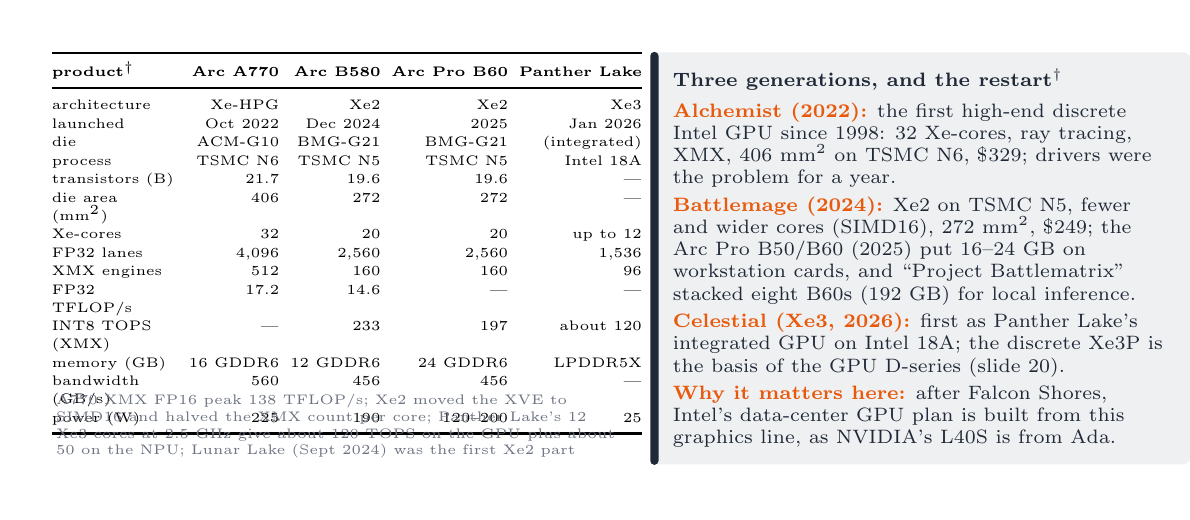
\begin{tikzpicture}
  \useasboundingbox (0,0) rectangle (14.4,5.9);
  \node[anchor=north west,inner sep=0,font=\fontsize{5.3}{6.4}\selectfont] at (0.3,5.6) {%
    \renewcommand{\arraystretch}{1.05}\setlength{\tabcolsep}{2.0pt}%
    \begin{tabular}{@{}>{\raggedright\arraybackslash}p{1.6cm}rrrr@{}}
      \toprule
      \textbf{product}$^\dagger$ & \textbf{Arc A770} & \textbf{Arc B580} & \textbf{Arc Pro B60} & \textbf{Panther Lake}\\
      \midrule
      architecture & Xe-HPG & Xe2 & Xe2 & Xe3\\
      launched & Oct 2022 & Dec 2024 & 2025 & Jan 2026\\
      die & ACM-G10 & BMG-G21 & BMG-G21 & (integrated)\\
      process & TSMC N6 & TSMC N5 & TSMC N5 & Intel 18A\\
      transistors (B) & 21.7 & 19.6 & 19.6 & ---\\
      die area (mm$^2$) & 406 & 272 & 272 & ---\\
      Xe-cores & 32 & 20 & 20 & up to 12\\
      FP32 lanes & 4{,}096 & 2{,}560 & 2{,}560 & 1{,}536\\
      XMX engines & 512 & 160 & 160 & 96\\
      FP32 TFLOP/s & 17.2 & 14.6 & --- & ---\\
      INT8 TOPS (XMX) & --- & 233 & 197 & about 120\\
      memory (GB) & 16 GDDR6 & 12 GDDR6 & 24 GDDR6 & LPDDR5X\\
      bandwidth (GB/s) & 560 & 456 & 456 & ---\\
      power (W) & 225 & 190 & 120--200 & 25\\
      \bottomrule
    \end{tabular}};
  \node[lab,font=\tiny,anchor=north west,text width=7.2cm] at (0.3,1.3) {A770 XMX FP16 peak 138 TFLOP/s; Xe2 moved the XVE to SIMD16 and halved the XMX count per core; Panther Lake's 12 Xe3 cores at 2.5 GHz give about 120 TOPS on the GPU plus about 50 on the NPU; Lunar Lake (Sept 2024) was the first Xe2 part};
  \bgpanels{7.9}{5.6}{6.3cm}{Three generations, and the restart$^\dagger$}{%
    \hl{attn}{Alchemist (2022):} the first high-end discrete Intel GPU
    since 1998: 32 Xe-cores, ray tracing, XMX, 406 mm$^2$ on TSMC
    N6, \$329; drivers were the problem for a year.\\[2pt]
    \hl{attn}{Battlemage (2024):} Xe2 on TSMC N5, fewer and wider
    cores (SIMD16), 272 mm$^2$, \$249; the Arc Pro B50/B60 (2025) put
    16--24 GB on workstation cards, and ``Project Battlematrix''
    stacked eight B60s (192 GB) for local inference.\\[2pt]
    \hl{attn}{Celestial (Xe3, 2026):} first as Panther Lake's
    integrated GPU on Intel 18A; the discrete Xe3P is the basis of
    the GPU D-series (slide 20).\\[2pt]
    \hl{attn}{Why it matters here:} after Falcon Shores, Intel's
    data-center GPU plan is built from this graphics line, as
    NVIDIA's L40S is from Ada.}
\end{tikzpicture}
\end{frame}

% ---------------------------------------------------------------- 16
\begin{frame}{Gaudi 2 and Gaudi 3: Intel's other accelerator}
\framesubtitle{The Habana architecture: matrix engines, tensor cores and Ethernet on the die; strong on paper, weak in the market.}
\centering
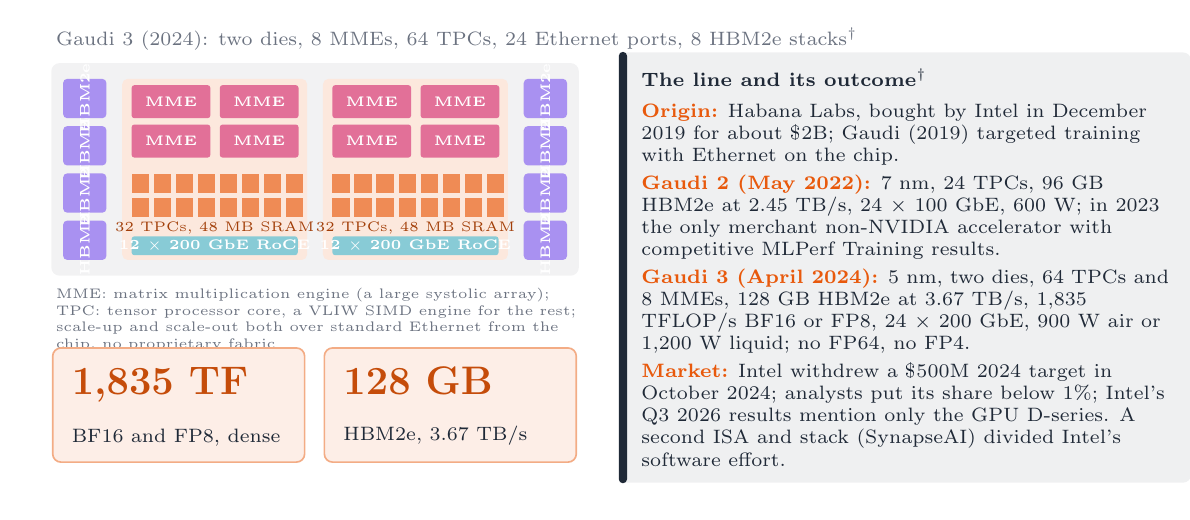
\begin{tikzpicture}
  \useasboundingbox (0,0) rectangle (14.4,5.9);
  \node[lab,anchor=south west] at (0.3,5.55) {Gaudi 3 (2024): two dies, 8 MMEs, 64 TPCs, 24 Ethernet ports, 8 HBM2e stacks$^\dagger$};
  \begin{scope}[shift={(0.3,2.75)}]
    \fill[ink!6,rounded corners=3pt] (0,0) rectangle (6.7,2.7);
    \foreach \s in {0,...,3}{\fill[posc!60,rounded corners=1.5pt] (0.15,0.2+\s*0.6) rectangle ++(0.55,0.5); \node[font=\fontsize{4.5}{5}\selectfont\bfseries,text=white,rotate=90] at (0.425,0.45+\s*0.6) {HBM2e};
      \fill[posc!60,rounded corners=1.5pt] (6.0,0.2+\s*0.6) rectangle ++(0.55,0.5); \node[font=\fontsize{4.5}{5}\selectfont\bfseries,text=white,rotate=90] at (6.275,0.45+\s*0.6) {HBM2e};}
    \foreach \d/\x in {0/0.9,1/3.45}{
      \fill[attn!14,rounded corners=2pt] (\x,0.2) rectangle (\x+2.35,2.5);
      \foreach \r in {0,1}{\foreach \c in {0,1}{\fill[outc!70,rounded corners=1pt] (\x+0.12+\c*1.12,1.5+\r*0.5) rectangle ++(1.0,0.42); \node[font=\fontsize{4.5}{5}\selectfont\bfseries,text=white] at (\x+0.62+\c*1.12,1.71+\r*0.5) {MME};}}
      \foreach \r in {0,1}{\foreach \c in {0,...,7}{\fill[attn!70] (\x+0.12+\c*0.28,0.75+\r*0.3) rectangle ++(0.22,0.24);}}
      \node[font=\fontsize{4.5}{5}\selectfont,text=attn!70!black] at (\x+1.175,0.6) {32 TPCs, 48 MB SRAM};
      \fill[vc!50,rounded corners=1pt] (\x+0.12,0.26) rectangle (\x+2.23,0.5); \node[font=\fontsize{4.5}{5}\selectfont\bfseries,text=white] at (\x+1.175,0.38) {12 $\times$ 200 GbE RoCE};}
  \end{scope}
  \node[lab,font=\tiny,anchor=north west,text width=6.7cm] at (0.3,2.65) {MME: matrix multiplication engine (a large systolic array); TPC: tensor processor core, a VLIW SIMD engine for the rest; scale-up and scale-out both over standard Ethernet from the chip, no proprietary fabric};
  \stat{0.3}{1.85}{1,835 TF}{BF16 and FP8, dense}{attn}
  \stat{3.75}{1.85}{128 GB}{HBM2e, 3.67 TB/s}{attn}
  \bgpanels{7.5}{5.6}{6.7cm}{The line and its outcome$^\dagger$}{%
    \hl{attn}{Origin:} Habana Labs, bought by Intel in December 2019
    for about \$2B; Gaudi (2019) targeted training with Ethernet on
    the chip.\\[2pt]
    \hl{attn}{Gaudi 2 (May 2022):} 7 nm, 24 TPCs, 96 GB HBM2e at 2.45
    TB/s, 24 $\times$ 100 GbE, 600 W; in 2023 the only merchant
    non-NVIDIA accelerator with competitive MLPerf Training results.\\[2pt]
    \hl{attn}{Gaudi 3 (April 2024):} 5 nm, two dies, 64 TPCs and 8
    MMEs, 128 GB HBM2e at 3.67 TB/s, 1{,}835 TFLOP/s BF16 or FP8, 24
    $\times$ 200 GbE, 900 W air or 1{,}200 W liquid; no FP64, no FP4.\\[2pt]
    \hl{attn}{Market:} Intel withdrew a \$500M 2024 target in October
    2024; analysts put its share below 1\%; Intel's Q3 2026 results
    mention only the GPU D-series. A second ISA and stack (SynapseAI)
    divided Intel's software effort.}
\end{tikzpicture}
\end{frame}

% ---------------------------------------------------------------- 17
\stage{5}
\begin{frame}{Ponte Vecchio: 47 active tiles from five process nodes}
\framesubtitle{Intel's exascale GPU (announced 2021, launched 2023) is the most complex package any vendor has shipped.}
\centering
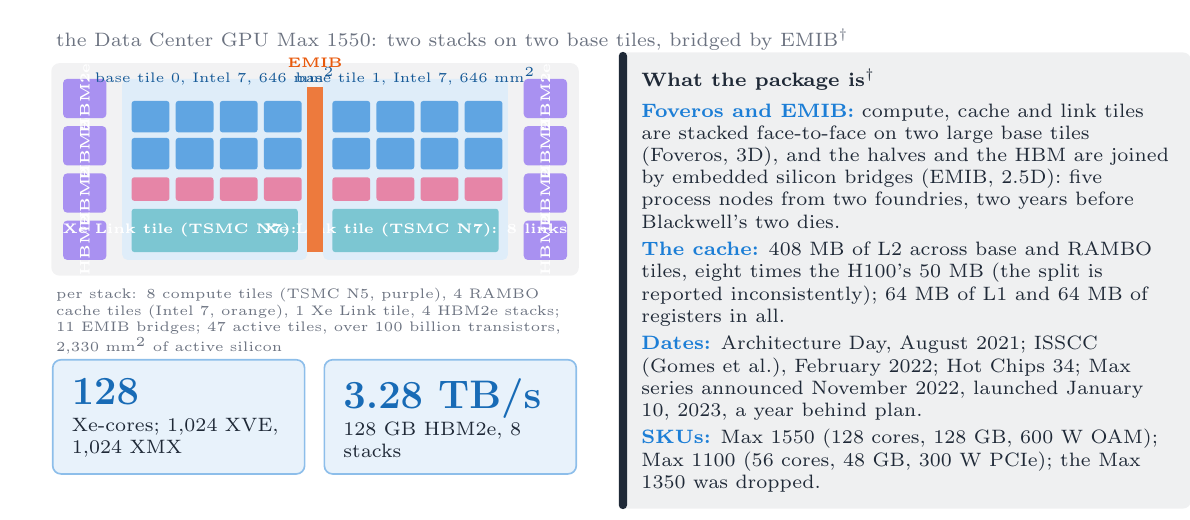
\begin{tikzpicture}
  \useasboundingbox (0,0) rectangle (14.4,5.9);
  \node[lab,anchor=south west] at (0.3,5.55) {the Data Center GPU Max 1550: two stacks on two base tiles, bridged by EMIB$^\dagger$};
  \begin{scope}[shift={(0.3,2.75)}]
    \fill[ink!6,rounded corners=3pt] (0,0) rectangle (6.7,2.7);
    \foreach \s in {0,...,3}{\fill[posc!60,rounded corners=1.5pt] (0.15,0.2+\s*0.6) rectangle ++(0.55,0.5); \node[font=\fontsize{4.5}{5}\selectfont\bfseries,text=white,rotate=90] at (0.425,0.45+\s*0.6) {HBM2e};
      \fill[posc!60,rounded corners=1.5pt] (6.0,0.2+\s*0.6) rectangle ++(0.55,0.5); \node[font=\fontsize{4.5}{5}\selectfont\bfseries,text=white,rotate=90] at (6.275,0.45+\s*0.6) {HBM2e};}
    \foreach \b/\x in {0/0.9,1/3.45}{
      \fill[mlp!14,rounded corners=2pt] (\x,0.2) rectangle (\x+2.35,2.5);
      \node[font=\fontsize{4.5}{5}\selectfont,text=mlp!70!black,anchor=south] at (\x+1.175,2.3) {base tile \b, Intel 7, 646 mm$^2$};
      \foreach \r in {0,1}{\foreach \c in {0,...,3}{\fill[mlp!70,rounded corners=1pt] (\x+0.12+\c*0.56,1.35+\r*0.47) rectangle ++(0.48,0.4);}}
      \foreach \c in {0,...,3}{\fill[outc!60,rounded corners=1pt] (\x+0.12+\c*0.56,0.95) rectangle ++(0.48,0.3);}
      \fill[vc!55,rounded corners=1pt] (\x+0.12,0.3) rectangle (\x+2.23,0.85); \node[font=\fontsize{4.5}{5}\selectfont\bfseries,text=white] at (\x+1.175,0.575) {Xe Link tile (TSMC N7): 8 links};}
    \fill[attn!80] (3.25,0.3) rectangle (3.45,2.4); \node[font=\fontsize{4.5}{5}\selectfont\bfseries,text=attn,anchor=south] at (3.35,2.52) {EMIB};
  \end{scope}
  \node[lab,font=\tiny,anchor=north west,text width=6.7cm] at (0.3,2.65) {per stack: 8 compute tiles (TSMC N5, purple), 4 RAMBO cache tiles (Intel 7, orange), 1 Xe Link tile, 4 HBM2e stacks; 11 EMIB bridges; 47 active tiles, over 100 billion transistors, 2{,}330 mm$^2$ of active silicon};
  \stat{0.3}{1.7}{128}{Xe-cores; 1{,}024 XVE, 1{,}024 XMX}{mlp}
  \stat{3.75}{1.7}{3.28 TB/s}{128 GB HBM2e, 8 stacks}{mlp}
  \bgpanels{7.5}{5.6}{6.7cm}{What the package is$^\dagger$}{%
    \hl{mlp}{Foveros and EMIB:} compute, cache and link tiles are
    stacked face-to-face on two large base tiles (Foveros, 3D), and
    the halves and the HBM are joined by embedded silicon bridges
    (EMIB, 2.5D): five process nodes from two foundries, two years
    before Blackwell's two dies.\\[2pt]
    \hl{mlp}{The cache:} 408 MB of L2 across base and RAMBO tiles,
    eight times the H100's 50 MB (the split is reported
    inconsistently); 64 MB of L1 and 64 MB of registers in all.\\[2pt]
    \hl{mlp}{Dates:} Architecture Day, August 2021; ISSCC (Gomes et
    al.), February 2022; Hot Chips 34; Max series announced November
    2022, launched January 10, 2023, a year behind plan.\\[2pt]
    \hl{mlp}{SKUs:} Max 1550 (128 cores, 128 GB, 600 W OAM); Max 1100
    (56 cores, 48 GB, 300 W PCIe); the Max 1350 was dropped.}
\end{tikzpicture}
\end{frame}

% ---------------------------------------------------------------- 18
\begin{frame}{The Xe-HPC core; the Max 1550 against its contemporaries}
\framesubtitle{Full-rate FP64, a 512 KB local store per core, a matrix engine a generation behind.}
\centering
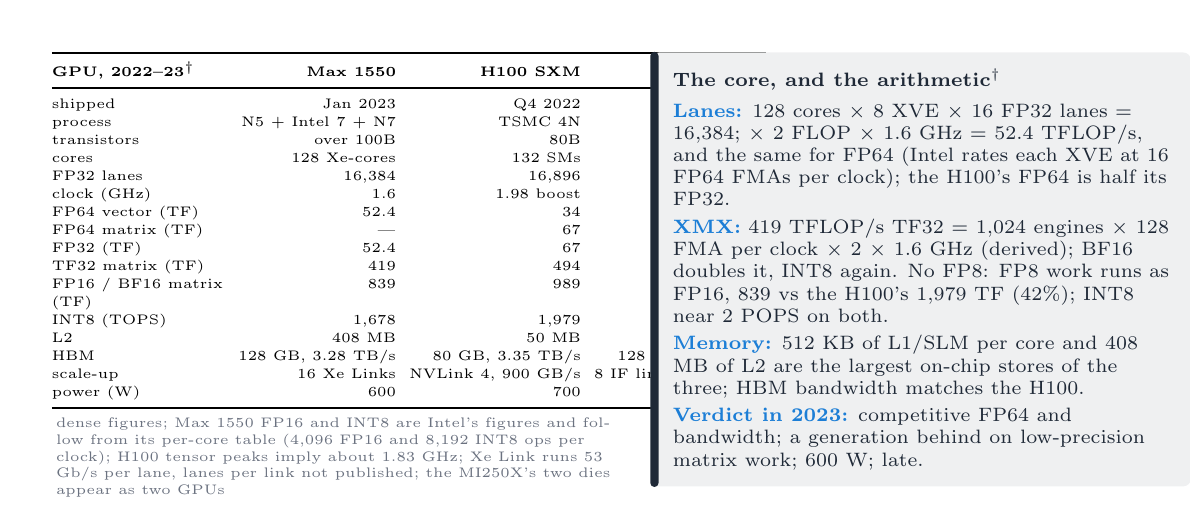
\begin{tikzpicture}
  \useasboundingbox (0,0) rectangle (14.4,5.9);
  \node[anchor=north west,inner sep=0,font=\fontsize{5.5}{6.5}\selectfont] at (0.3,5.6) {%
    \renewcommand{\arraystretch}{1.0}\setlength{\tabcolsep}{2.4pt}%
    \begin{tabular}{@{}>{\raggedright\arraybackslash}p{2.2cm}rrr@{}}
      \toprule
      \textbf{GPU, 2022--23}$^\dagger$ & \textbf{Max 1550} & \textbf{H100 SXM} & \textbf{MI250X}\\
      \midrule
      shipped & Jan 2023 & Q4 2022 & Nov 2021\\
      process & N5 $+$ Intel 7 $+$ N7 & TSMC 4N & TSMC N6\\
      transistors & over 100B & 80B & 58.2B\\
      cores & 128 Xe-cores & 132 SMs & 220 CUs\\
      FP32 lanes & 16{,}384 & 16{,}896 & 14{,}080\\
      clock (GHz) & 1.6 & 1.98 boost & 1.7\\
      FP64 vector (TF) & 52.4 & 34 & 47.9\\
      FP64 matrix (TF) & --- & 67 & 95.7\\
      FP32 (TF) & 52.4 & 67 & 47.9\\
      TF32 matrix (TF) & 419 & 494 & ---\\
      FP16 / BF16 matrix (TF) & 839 & 989 & 383\\
      INT8 (TOPS) & 1{,}678 & 1{,}979 & 383\\
      L2 & 408 MB & 50 MB & 2 $\times$ 8 MB\\
      HBM & 128 GB, 3.28 TB/s & 80 GB, 3.35 TB/s & 128 GB, 3.2 TB/s\\
      scale-up & 16 Xe Links & NVLink 4, 900 GB/s & 8 IF links, 800 GB/s\\
      power (W) & 600 & 700 & 560\\
      \bottomrule
    \end{tabular}};
  \node[lab,font=\tiny,anchor=north west,text width=7.2cm] at (0.3,1.0) {dense figures; Max 1550 FP16 and INT8 are Intel's figures and follow from its per-core table (4{,}096 FP16 and 8{,}192 INT8 ops per clock); H100 tensor peaks imply about 1.83 GHz; Xe Link runs 53 Gb/s per lane, lanes per link not published; the MI250X's two dies appear as two GPUs};
  \bgpanels{7.9}{5.6}{6.3cm}{The core, and the arithmetic$^\dagger$}{%
    \hl{mlp}{Lanes:} 128 cores $\times$ 8 XVE $\times$ 16 FP32 lanes
    $=$ 16{,}384; $\times$ 2 FLOP $\times$ 1.6 GHz $=$ 52.4 TFLOP/s,
    and the same for FP64 (Intel rates each XVE at 16 FP64 FMAs per
    clock); the H100's FP64 is half its FP32.\\[2pt]
    \hl{mlp}{XMX:} 419 TFLOP/s TF32 $=$ 1{,}024 engines $\times$ 128
    FMA per clock $\times$ 2 $\times$ 1.6 GHz (derived); BF16 doubles
    it, INT8 again. No FP8: FP8 work runs as FP16, 839 vs the
    H100's 1{,}979 TF (42\%); INT8 near 2 POPS on both.\\[2pt]
    \hl{mlp}{Memory:} 512 KB of L1/SLM per core and 408 MB of L2 are
    the largest on-chip stores of the three; HBM bandwidth matches
    the H100.\\[2pt]
    \hl{mlp}{Verdict in 2023:} competitive FP64 and bandwidth; a
    generation behind on low-precision matrix work; 600 W; late.}
\end{tikzpicture}
\end{frame}

% ---------------------------------------------------------------- 19
\begin{frame}{Aurora: 63,744 GPUs, 1.012 exaflops, 38.7 MW}
\framesubtitle{Planned in 2015 for 2018; delivered in 2023 with Ponte Vecchio; exascale HPL on Intel GPUs in 2024.}
\centering
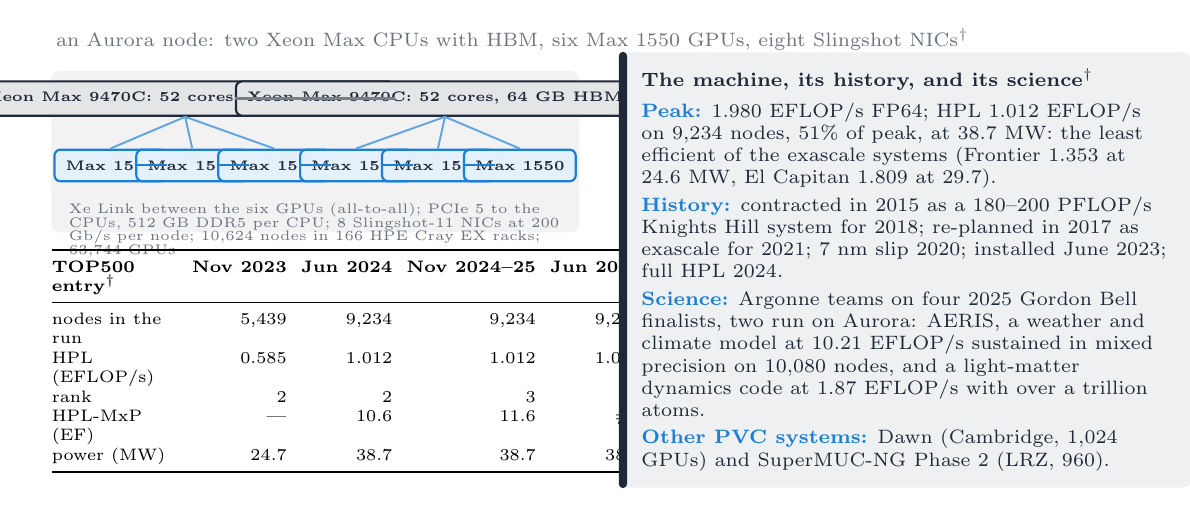
\begin{tikzpicture}
  \useasboundingbox (0,0) rectangle (14.4,5.9);
  \node[lab,anchor=south west] at (0.3,5.55) {an Aurora node: two Xeon Max CPUs with HBM, six Max 1550 GPUs, eight Slingshot NICs$^\dagger$};
  \begin{scope}[shift={(0.3,3.3)}]
    \fill[ink!6,rounded corners=3pt] (0,0) rectangle (6.7,2.05);
    \foreach \c/\x in {0/1.7,1/5.0}{\node[comp=ink,minimum width=2.9cm,minimum height=0.42cm,font=\fontsize{4.5}{5}\selectfont\bfseries,text=ink] (c\c) at (\x,1.7) {Xeon Max 9470C: 52 cores, 64 GB HBM2e};}
    \draw[ink!60,line width=0.8pt] (c0) -- (c1);
    \foreach \g in {0,...,5}{\node[comp=mlp,minimum width=0.8cm,minimum height=0.4cm,font=\fontsize{4.5}{5}\selectfont\bfseries,text=ink] (g\g) at (0.75+\g*1.04,0.85) {Max 1550};}
    \foreach \g in {0,1,2}{\draw[mlp!70,line width=0.7pt] (c0.south) -- (g\g.north);} \foreach \g in {3,4,5}{\draw[mlp!70,line width=0.7pt] (c1.south) -- (g\g.north);}
    \foreach \g in {0,...,4}{\pgfmathtruncatemacro{\h}{\g+1}\draw[mlp,line width=0.7pt] (g\g) -- (g\h);}
    \node[font=\fontsize{4.5}{5}\selectfont,text=muted,anchor=north west,text width=6.5cm] at (0.1,0.5) {Xe Link between the six GPUs (all-to-all); PCIe 5 to the CPUs, 512 GB DDR5 per CPU; 8 Slingshot-11 NICs at 200 Gb/s per node; 10{,}624 nodes in 166 HPE Cray EX racks; 63{,}744 GPUs};
  \end{scope}
  \node[anchor=north west,inner sep=0,font=\fontsize{5.7}{6.8}\selectfont] at (0.3,3.1) {%
    \renewcommand{\arraystretch}{1.05}\setlength{\tabcolsep}{2.6pt}%
    \begin{tabular}{@{}>{\raggedright\arraybackslash}p{1.6cm}rrrr@{}}
      \toprule
      \textbf{TOP500 entry}$^\dagger$ & \textbf{Nov 2023} & \textbf{Jun 2024} & \textbf{Nov 2024--25} & \textbf{Jun 2026}\\
      \midrule
      nodes in the run & 5{,}439 & 9{,}234 & 9{,}234 & 9{,}234\\
      HPL (EFLOP/s) & 0.585 & 1.012 & 1.012 & 1.012\\
      rank & 2 & 2 & 3 & 4\\
      HPL-MxP (EF) & --- & 10.6 & 11.6 & \#3\\
      power (MW) & 24.7 & 38.7 & 38.7 & 38.7\\
      \bottomrule
    \end{tabular}};
  \bgpanels{7.5}{5.6}{6.7cm}{The machine, its history, and its science$^\dagger$}{%
    \hl{mlp}{Peak:} 1.980 EFLOP/s FP64; HPL 1.012 EFLOP/s on 9{,}234
    nodes, 51\% of peak, at 38.7 MW: the least efficient of the
    exascale systems (Frontier 1.353 at 24.6 MW, El Capitan 1.809 at
    29.7).\\[2pt]
    \hl{mlp}{History:} contracted in 2015 as a 180--200 PFLOP/s Knights
    Hill system for 2018; re-planned in 2017 as exascale for 2021;
    7 nm slip 2020; installed June 2023; full HPL 2024.\\[2pt]
    \hl{mlp}{Science:} Argonne teams on four 2025 Gordon Bell
    finalists, two run on Aurora: AERIS, a weather and climate model
    at 10.21 EFLOP/s sustained in mixed precision on 10{,}080 nodes,
    and a light-matter dynamics code at 1.87 EFLOP/s with over a
    trillion atoms.\\[2pt]
    \hl{mlp}{Other PVC systems:} Dawn (Cambridge, 1{,}024 GPUs) and
    SuperMUC-NG Phase 2 (LRZ, 960).}
\end{tikzpicture}
\end{frame}

% ---------------------------------------------------------------- 20
\begin{frame}{After Ponte Vecchio: cancellations and a restart from Xe3}
\framesubtitle{Rialto Bridge and Falcon Shores were cancelled; Jaguar Shores has no date; the GPU D-series is sampling.}
\centering
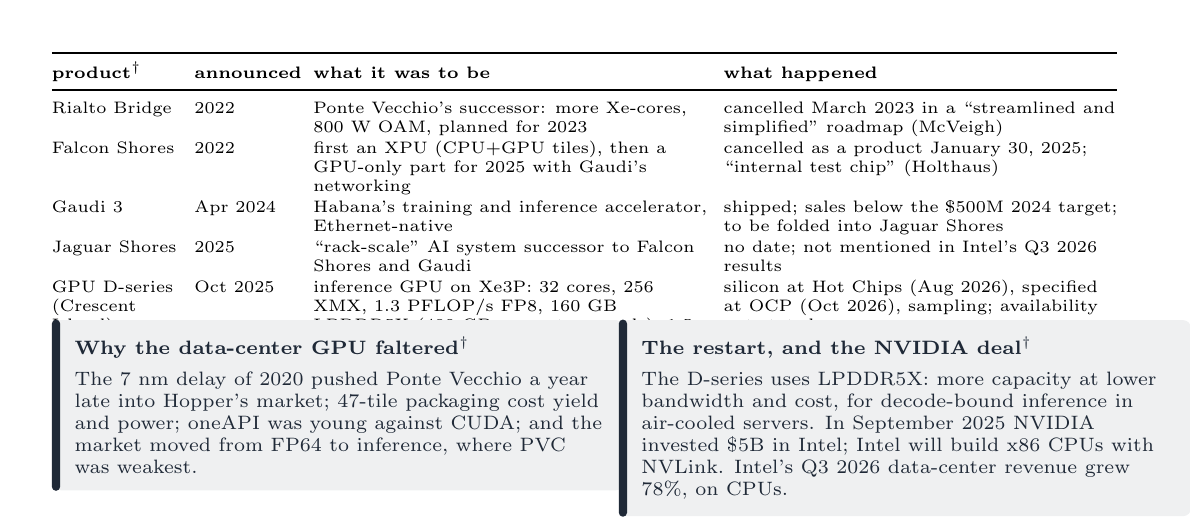
\begin{tikzpicture}
  \useasboundingbox (0,0) rectangle (14.4,5.9);
  \node[anchor=north west,inner sep=0,font=\fontsize{5.8}{6.9}\selectfont] at (0.3,5.6) {%
    \renewcommand{\arraystretch}{1.1}\setlength{\tabcolsep}{3.0pt}%
    \begin{tabular}{@{}>{\raggedright\arraybackslash}p{1.6cm}>{\raggedright\arraybackslash}p{1.3cm}>{\raggedright\arraybackslash}p{5.0cm}>{\raggedright\arraybackslash}p{5.0cm}@{}}
      \toprule
      \textbf{product}$^\dagger$ & \textbf{announced} & \textbf{what it was to be} & \textbf{what happened}\\
      \midrule
      Rialto Bridge & 2022 & Ponte Vecchio's successor: more Xe-cores, 800 W OAM, planned for 2023 & cancelled March 2023 in a ``streamlined and simplified'' roadmap (McVeigh)\\
      Falcon Shores & 2022 & first an XPU (CPU$+$GPU tiles), then a GPU-only part for 2025 with Gaudi's networking & cancelled as a product January 30, 2025; ``internal test chip'' (Holthaus)\\
      Gaudi 3 & Apr 2024 & Habana's training and inference accelerator, Ethernet-native & shipped; sales below the \$500M 2024 target; to be folded into Jaguar Shores\\
      Jaguar Shores & 2025 & ``rack-scale'' AI system successor to Falcon Shores and Gaudi & no date; not mentioned in Intel's Q3 2026 results\\
      GPU D-series (Crescent Island) & Oct 2025 & inference GPU on Xe3P: 32 cores, 256 XMX, 1.3 PFLOP/s FP8, 160 GB LPDDR5X (480 GB on partner cards), 1.5 TB/s, 350 W PCIe & silicon at Hot Chips (Aug 2026), specified at OCP (Oct 2026), sampling; availability not stated\\
      \bottomrule
    \end{tabular}};
  \bgpanels{0.3}{2.2}{6.7cm}{Why the data-center GPU faltered$^\dagger$}{%
    The 7 nm delay of 2020 pushed Ponte Vecchio a year late into
    Hopper's market; 47-tile packaging cost yield and power; oneAPI
    was young against CUDA; and the market moved from FP64 to
    inference, where PVC was weakest.}
  \bgpanels{7.5}{2.2}{6.7cm}{The restart, and the NVIDIA deal$^\dagger$}{%
    The D-series uses LPDDR5X: more capacity at lower bandwidth and
    cost, for decode-bound inference in air-cooled servers. In
    September 2025 NVIDIA invested \$5B in Intel; Intel will build
    x86 CPUs with NVLink. Intel's Q3 2026 data-center revenue grew
    78\%, on CPUs.}
\end{tikzpicture}
\end{frame}

% ---------------------------------------------------------------- 21
\stage{6}
\begin{frame}{Scale-up fabrics: NVLink, Infinity Fabric, Xe Link, UALink}
\framesubtitle{The link between GPUs is NVIDIA's widest lead; AMD answered with a standard, Intel with Xe Link.}
\centering
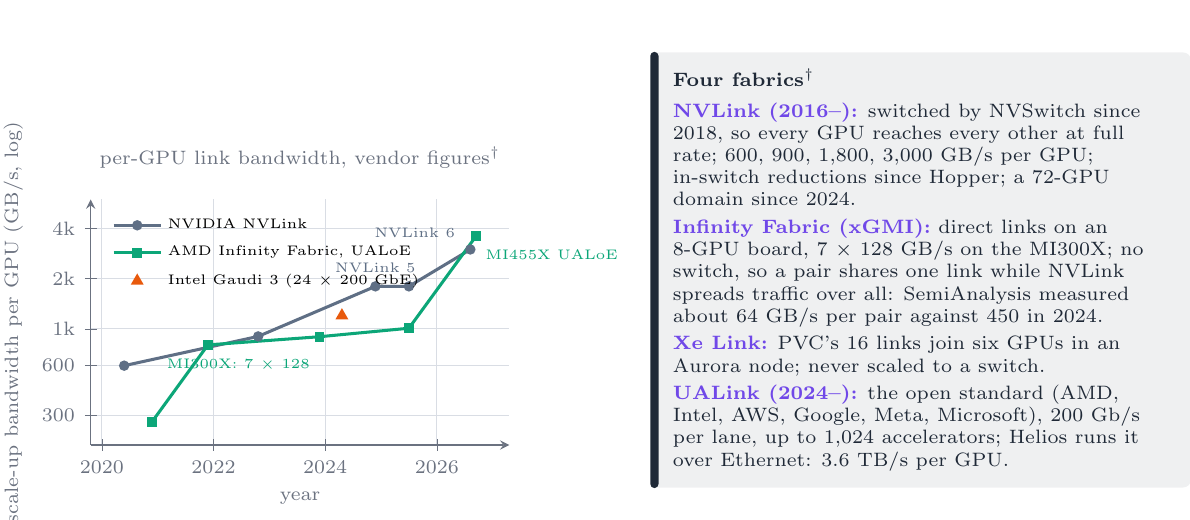
\begin{tikzpicture}
  \useasboundingbox (0,0) rectangle (14.4,5.9);
  \begin{scope}[shift={(0.8,0.6)}]
  \begin{axis}[lecture,width=6.9cm,height=4.7cm,ymode=log,xmin=2019.8,xmax=2027.3,ymin=200,ymax=6000,
      xlabel={year},ylabel={scale-up bandwidth per GPU (GB/s, log)},
      xtick={2020,2022,2024,2026},xticklabel style={/pgf/number format/1000 sep={}},scaled x ticks=false,
      ytick={300,600,1000,2000,4000},yticklabels={300,600,1k,2k,4k},
      legend style={at={(0.03,0.97)},anchor=north west,font=\tiny},
      title style={font=\scriptsize,text=muted,at={(0.5,1.02)}},title={per-GPU link bandwidth, vendor figures$^\dagger$}]
    \addplot[tok,line width=1.1pt,mark=*,mark size=1.3pt] coordinates {(2020.4,600) (2022.8,900) (2024.9,1800) (2025.5,1800) (2026.6,3000)};
    \addlegendentry{NVIDIA NVLink}
    \addplot[emb,line width=1.1pt,mark=square*,mark size=1.2pt] coordinates {(2020.9,276) (2021.9,800) (2023.9,896) (2025.5,1008) (2026.7,3600)};
    \addlegendentry{AMD Infinity Fabric, UALoE}
    \addplot[attn,line width=1.1pt,mark=triangle*,mark size=1.6pt,only marks] coordinates {(2024.3,1200)};
    \addlegendentry{Intel Gaudi 3 (24 $\times$ 200 GbE)}
    \node[font=\tiny,text=tok,anchor=south east] at (axis cs:2026.5,3100) {NVLink 6};
    \node[font=\tiny,text=emb,anchor=north west] at (axis cs:2026.7,3400) {MI455X UALoE};
    \node[font=\tiny,text=emb,anchor=north east] at (axis cs:2023.9,750) {MI300X: 7 $\times$ 128};
    \node[font=\tiny,text=tok,anchor=south] at (axis cs:2024.9,1900) {NVLink 5};
  \end{axis}
  \end{scope}
  \bgpanels{7.9}{5.6}{6.3cm}{Four fabrics$^\dagger$}{%
    \hl{posc}{NVLink (2016--):} switched by NVSwitch since 2018, so
    every GPU reaches every other at full rate; 600, 900, 1{,}800,
    3{,}000 GB/s per GPU; in-switch reductions since Hopper; a 72-GPU
    domain since 2024.\\[2pt]
    \hl{posc}{Infinity Fabric (xGMI):} direct links on an 8-GPU
    board, 7 $\times$ 128 GB/s on the MI300X; no switch, so a pair
    shares one link while NVLink spreads traffic over all:
    SemiAnalysis measured about 64 GB/s per pair against 450 in
    2024.\\[2pt]
    \hl{posc}{Xe Link:} PVC's 16 links join six GPUs in an Aurora
    node; never scaled to a switch.\\[2pt]
    \hl{posc}{UALink (2024--):} the open standard (AMD, Intel, AWS,
    Google, Meta, Microsoft), 200 Gb/s per lane, up to 1{,}024
    accelerators; Helios runs it over Ethernet: 3.6 TB/s per GPU.}
\end{tikzpicture}
\end{frame}

% ---------------------------------------------------------------- 22
\begin{frame}{Rack-scale: the NVL72 family against Helios}
\framesubtitle{Both sell 72-GPU liquid-cooled racks with their own CPUs; AMD's is wider, holds more HBM, shipped later.}
\centering
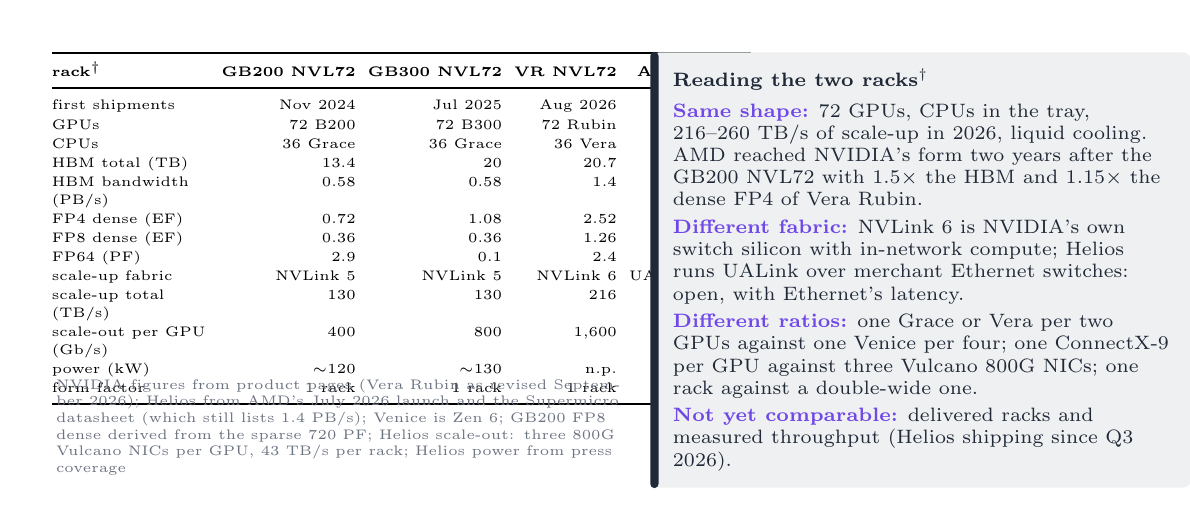
\begin{tikzpicture}
  \useasboundingbox (0,0) rectangle (14.4,5.9);
  \node[anchor=north west,inner sep=0,font=\fontsize{5.5}{6.5}\selectfont] at (0.3,5.6) {%
    \renewcommand{\arraystretch}{1.06}\setlength{\tabcolsep}{2.2pt}%
    \begin{tabular}{@{}>{\raggedright\arraybackslash}p{2.0cm}rrrr@{}}
      \toprule
      \textbf{rack}$^\dagger$ & \textbf{GB200 NVL72} & \textbf{GB300 NVL72} & \textbf{VR NVL72} & \textbf{AMD Helios}\\
      \midrule
      first shipments & Nov 2024 & Jul 2025 & Aug 2026 & Q3 2026\\
      GPUs & 72 B200 & 72 B300 & 72 Rubin & 72 MI455X\\
      CPUs & 36 Grace & 36 Grace & 36 Vera & 18 Venice\\
      HBM total (TB) & 13.4 & 20 & 20.7 & 31\\
      HBM bandwidth (PB/s) & 0.58 & 0.58 & 1.4 & 1.7\\
      FP4 dense (EF) & 0.72 & 1.08 & 2.52 & 2.9\\
      FP8 dense (EF) & 0.36 & 0.36 & 1.26 & 1.4\\
      FP64 (PF) & 2.9 & 0.1 & 2.4 & n.p.\\
      scale-up fabric & NVLink 5 & NVLink 5 & NVLink 6 & UALink (Eth.)\\
      scale-up total (TB/s) & 130 & 130 & 216 & 260\\
      scale-out per GPU (Gb/s) & 400 & 800 & 1{,}600 & 2{,}400\\
      power (kW) & ${\sim}$120 & ${\sim}$130 & n.p. & 225--245\\
      form factor & 1 rack & 1 rack & 1 rack & 2 wide\\
      \bottomrule
    \end{tabular}};
  \node[lab,font=\tiny,anchor=north west,text width=7.2cm] at (0.3,1.5) {NVIDIA figures from product pages (Vera Rubin as revised September 2026); Helios from AMD's July 2026 launch and the Supermicro datasheet (which still lists 1.4 PB/s); Venice is Zen 6; GB200 FP8 dense derived from the sparse 720 PF; Helios scale-out: three 800G Vulcano NICs per GPU, 43 TB/s per rack; Helios power from press coverage};
  \bgpanels{7.9}{5.6}{6.3cm}{Reading the two racks$^\dagger$}{%
    \hl{posc}{Same shape:} 72 GPUs, CPUs in the tray, 216--260 TB/s
    of scale-up in 2026, liquid cooling. AMD reached NVIDIA's form
    two years after the GB200 NVL72 with 1.5$\times$ the HBM and
    1.15$\times$ the dense FP4 of Vera Rubin.\\[2pt]
    \hl{posc}{Different fabric:} NVLink 6 is NVIDIA's own switch
    silicon with in-network compute; Helios runs UALink over
    merchant Ethernet switches: open, with Ethernet's latency.\\[2pt]
    \hl{posc}{Different ratios:} one Grace or Vera per two GPUs
    against one Venice per four; one ConnectX-9 per GPU against
    three Vulcano 800G NICs; one rack against a double-wide one.\\[2pt]
    \hl{posc}{Not yet comparable:} delivered racks and measured
    throughput (Helios shipping since Q3 2026).}
\end{tikzpicture}
\end{frame}

% ---------------------------------------------------------------- 23
\begin{frame}{Standards: OAM, UBB, UALink, Ultra Ethernet, NVLink Fusion}
\framesubtitle{Everyone but NVIDIA builds on open form factors and fabrics; NVIDIA opened its fabric to partners instead.}
\centering
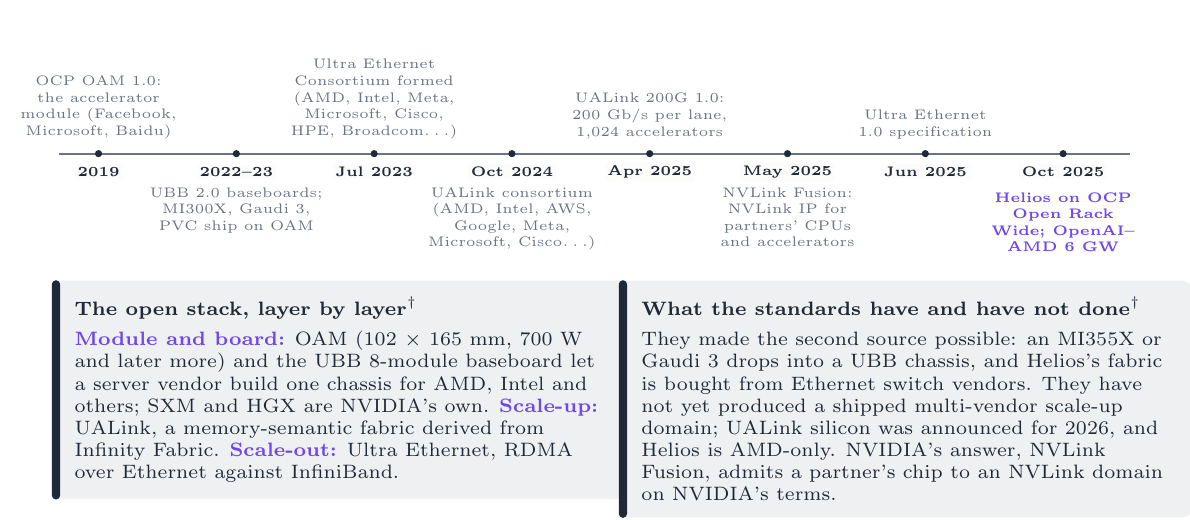
\begin{tikzpicture}
  \useasboundingbox (0,0) rectangle (14.4,5.9);
  \draw[muted,line width=0.8pt] (0.4,4.3) -- (14.0,4.3);
  \foreach \x in {0.9,2.65,4.4,6.15,7.9,9.65,11.4,13.15}{\fill[ink] (\x,4.3) circle (1.3pt);}
  \foreach \yr/\x in {2019/0.9,2022--23/2.65,Jul 2023/4.4,Oct 2024/6.15,Apr 2025/7.9,May 2025/9.65,Jun 2025/11.4,Oct 2025/13.15}{\node[font=\tiny\bfseries,text=ink,fill=paper,inner sep=1pt] at (\x,4.07) {\yr};}
  \node[lab,anchor=south,text width=2.4cm,align=center,font=\tiny] at (0.9,4.43) {OCP OAM 1.0: the accelerator module (Facebook, Microsoft, Baidu)};
  \node[lab,anchor=north,text width=2.4cm,align=center,font=\tiny] at (2.65,3.93) {UBB 2.0 baseboards; MI300X, Gaudi 3, PVC ship on OAM};
  \node[lab,anchor=south,text width=2.4cm,align=center,font=\tiny] at (4.4,4.43) {Ultra Ethernet Consortium formed (AMD, Intel, Meta, Microsoft, Cisco, HPE, Broadcom$\ldots$)};
  \node[lab,anchor=north,text width=2.4cm,align=center,font=\tiny] at (6.15,3.93) {UALink consortium (AMD, Intel, AWS, Google, Meta, Microsoft, Cisco$\ldots$)};
  \node[lab,anchor=south,text width=2.4cm,align=center,font=\tiny] at (7.9,4.43) {UALink 200G 1.0: 200 Gb/s per lane, 1{,}024 accelerators};
  \node[lab,anchor=north,text width=2.4cm,align=center,font=\tiny] at (9.65,3.93) {NVLink Fusion: NVLink IP for partners' CPUs and accelerators};
  \node[lab,anchor=south,text width=2.4cm,align=center,font=\tiny] at (11.4,4.43) {Ultra Ethernet 1.0 specification};
  \node[anchor=north,text width=2.4cm,align=center,font=\tiny\bfseries,text=posc] at (13.15,3.93) {Helios on OCP Open Rack Wide; OpenAI--AMD 6 GW};
  \bgpanels{0.3}{2.7}{6.7cm}{The open stack, layer by layer$^\dagger$}{%
    \hl{posc}{Module and board:} OAM (102 $\times$ 165 mm, 700 W and
    later more) and the UBB 8-module baseboard let a server vendor
    build one chassis for AMD, Intel and others; SXM and HGX are
    NVIDIA's own. \hl{posc}{Scale-up:} UALink, a memory-semantic
    fabric derived from Infinity Fabric. \hl{posc}{Scale-out:} Ultra
    Ethernet, RDMA over Ethernet against InfiniBand.}
  \bgpanels{7.5}{2.7}{6.7cm}{What the standards have and have not done$^\dagger$}{%
    They made the second source possible: an MI355X or Gaudi 3 drops
    into a UBB chassis, and Helios's fabric is bought from Ethernet
    switch vendors. They have not yet produced a shipped
    multi-vendor scale-up domain; UALink silicon was announced for
    2026, and Helios is AMD-only. NVIDIA's answer, NVLink Fusion,
    admits a partner's chip to an NVLink domain on NVIDIA's terms.}
\end{tikzpicture}
\end{frame}

% ---------------------------------------------------------------- 24
\stage{7}
\begin{frame}{CUDA, ROCm and HIP, oneAPI and SYCL: three stacks}
\framesubtitle{The same layers in each stack: driver, compiler, libraries, frameworks; what differs is age and breadth.}
\centering
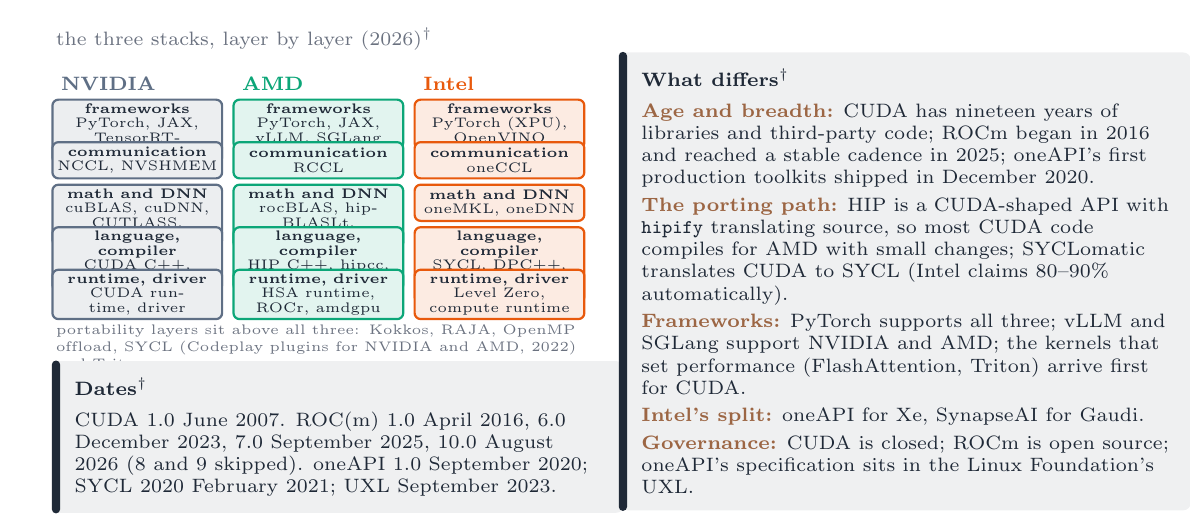
\begin{tikzpicture}
  \useasboundingbox (0,0) rectangle (14.4,5.9);
  \node[lab,anchor=south west] at (0.3,5.55) {the three stacks, layer by layer (2026)$^\dagger$};
  \foreach \c/\x/\name/\col in {0/0.3/{NVIDIA}/tok, 1/2.6/{AMD}/emb, 2/4.9/{Intel}/attn}{
    \node[font=\scriptsize\bfseries,text=\col,anchor=north west] at (\x,5.4) {\name};}
  \foreach \r/\y/\lab/\a/\b/\cc in {
      0/5.0/{frameworks}/{PyTorch, JAX, TensorRT-LLM, vLLM}/{PyTorch, JAX, vLLM, SGLang}/{PyTorch (XPU), OpenVINO},
      1/4.46/{communication}/{NCCL, NVSHMEM}/{RCCL}/{oneCCL},
      2/3.92/{math and DNN}/{cuBLAS, cuDNN, CUTLASS, TensorRT}/{rocBLAS, hipBLASLt, MIOpen, CK}/{oneMKL, oneDNN},
      3/3.38/{language, compiler}/{CUDA C++, nvcc, PTX; Triton}/{HIP C++, hipcc, LLVM; Triton}/{SYCL, DPC++, OpenMP; SYCLomatic},
      4/2.84/{runtime, driver}/{CUDA runtime, driver}/{HSA runtime, ROCr, amdgpu}/{Level Zero, compute runtime}}{
    \node[comp=tok,minimum width=2.15cm,minimum height=0.46cm,font=\fontsize{4.6}{5.2}\selectfont,text=ink,align=center,anchor=north west,text width=2.05cm,inner sep=1.5pt] at (0.3,\y) {\textbf{\lab}\\\a};
    \node[comp=emb,minimum width=2.15cm,minimum height=0.46cm,font=\fontsize{4.6}{5.2}\selectfont,text=ink,align=center,anchor=north west,text width=2.05cm,inner sep=1.5pt] at (2.6,\y) {\textbf{\lab}\\\b};
    \node[comp=attn,minimum width=2.15cm,minimum height=0.46cm,font=\fontsize{4.6}{5.2}\selectfont,text=ink,align=center,anchor=north west,text width=2.05cm,inner sep=1.5pt] at (4.9,\y) {\textbf{\lab}\\\cc};}
  \node[lab,font=\tiny,anchor=north west,text width=6.7cm] at (0.3,2.18) {portability layers sit above all three: Kokkos, RAJA, OpenMP offload, SYCL (Codeplay plugins for NVIDIA and AMD, 2022) and Triton};
  \bgpanels{0.3}{1.68}{6.7cm}{Dates$^\dagger$}{%
    CUDA 1.0 June 2007. ROC(m) 1.0 April 2016, 6.0 December 2023, 7.0
    September 2025, 10.0 August 2026 (8 and 9 skipped). oneAPI 1.0
    September 2020; SYCL 2020 February 2021; UXL September 2023.}
  \bgpanels{7.5}{5.6}{6.7cm}{What differs$^\dagger$}{%
    \hl{trn}{Age and breadth:} CUDA has nineteen years of libraries
    and third-party code; ROCm began in 2016 and reached a stable
    cadence in 2025; oneAPI's first production toolkits shipped in
    December 2020.\\[2pt]
    \hl{trn}{The porting path:} HIP is a CUDA-shaped API with
    \texttt{hipify} translating source, so most CUDA code compiles
    for AMD with small changes; SYCLomatic translates CUDA to SYCL
    (Intel claims 80--90\% automatically).\\[2pt]
    \hl{trn}{Frameworks:} PyTorch supports all three; vLLM and SGLang
    support NVIDIA and AMD; the kernels that set performance
    (FlashAttention, Triton) arrive first for CUDA.\\[2pt]
    \hl{trn}{Intel's split:} oneAPI for Xe, SynapseAI for Gaudi.\\[2pt]
    \hl{trn}{Governance:} CUDA is closed; ROCm is open source;
    oneAPI's specification sits in the Linux Foundation's UXL.}
\end{tikzpicture}
\end{frame}

% ---------------------------------------------------------------- 25
\begin{frame}{Portability: what the SYCL and Kokkos studies measure}
\framesubtitle{HPC codes run on all three vendors through portability layers; the gaps are in maturity, not the model.}
\centering
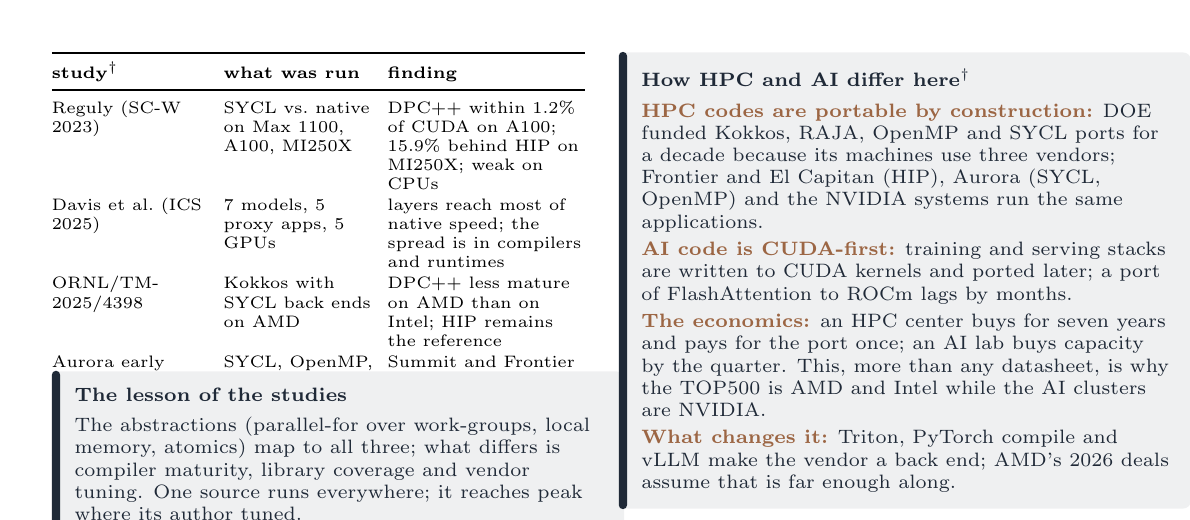
\begin{tikzpicture}
  \useasboundingbox (0,0) rectangle (14.4,5.9);
  \node[anchor=north west,inner sep=0,font=\fontsize{5.8}{6.9}\selectfont] at (0.3,5.6) {%
    \renewcommand{\arraystretch}{1.1}\setlength{\tabcolsep}{2.6pt}%
    \begin{tabular}{@{}>{\raggedright\arraybackslash}p{2.0cm}>{\raggedright\arraybackslash}p{1.9cm}>{\raggedright\arraybackslash}p{2.5cm}@{}}
      \toprule
      \textbf{study}$^\dagger$ & \textbf{what was run} & \textbf{finding}\\
      \midrule
      Reguly (SC-W 2023) & SYCL vs.\ native on Max 1100, A100, MI250X & DPC++ within 1.2\% of CUDA on A100; 15.9\% behind HIP on MI250X; weak on CPUs\\
      Davis et al.\ (ICS 2025) & 7 models, 5 proxy apps, 5 GPUs & layers reach most of native speed; the spread is in compilers and runtimes\\
      ORNL/TM-2025/4398 & Kokkos with SYCL back ends on AMD & DPC++ less mature on AMD than on Intel; HIP remains the reference\\
      Aurora early science (2023--25) & SYCL, OpenMP, Kokkos ports of DOE codes & Summit and Frontier codes ran; tuning for the 512 KB SLM and two stacks took the time\\
      \bottomrule
    \end{tabular}};
  \bgpanels{0.3}{1.55}{6.7cm}{The lesson of the studies}{%
    The abstractions (parallel-for over work-groups, local memory,
    atomics) map to all three; what differs is compiler maturity,
    library coverage and vendor tuning. One source runs everywhere;
    it reaches peak where its author tuned.}
  \bgpanels{7.5}{5.6}{6.7cm}{How HPC and AI differ here$^\dagger$}{%
    \hl{trn}{HPC codes are portable by construction:} DOE funded
    Kokkos, RAJA, OpenMP and SYCL ports for a decade because its
    machines use three vendors; Frontier and El Capitan (HIP), Aurora
    (SYCL, OpenMP) and the NVIDIA systems run the same applications.\\[2pt]
    \hl{trn}{AI code is CUDA-first:} training and serving stacks are
    written to CUDA kernels and ported later; a port of
    FlashAttention to ROCm lags by months.\\[2pt]
    \hl{trn}{The economics:} an HPC center buys for seven years and
    pays for the port once; an AI lab buys capacity by the quarter.
    This, more than any datasheet, is why the TOP500 is AMD and Intel
    while the AI clusters are NVIDIA.\\[2pt]
    \hl{trn}{What changes it:} Triton, PyTorch compile and vLLM make
    the vendor a back end; AMD's 2026 deals assume that is far enough
    along.}
\end{tikzpicture}
\end{frame}

% ---------------------------------------------------------------- 26
\begin{frame}{Achieved against peak: the software gap in numbers}
\framesubtitle{In 2024 independent tests put MI300X matrix multiply at half its peak, the H100 at three quarters.}
\centering
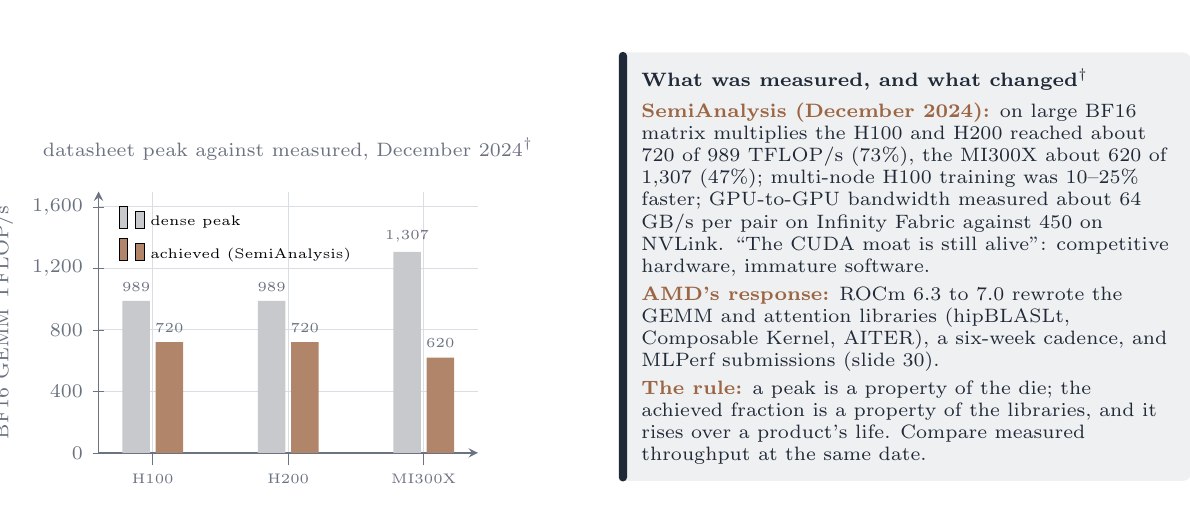
\begin{tikzpicture}
  \useasboundingbox (0,0) rectangle (14.4,5.9);
  \begin{scope}[shift={(0.9,0.5)}]
  \begin{axis}[lecture,width=6.4cm,height=4.9cm,ybar,bar width=10pt,ymin=0,ymax=1700,enlarge x limits=0.2,
      symbolic x coords={H100,H200,MI300X},xtick=data,xticklabel style={font=\tiny},
      ylabel={BF16 GEMM TFLOP/s},ytick={0,400,800,1200,1600},
      legend style={at={(0.03,0.97)},anchor=north west,font=\tiny},
      nodes near coords,nodes near coords style={font=\tiny,text=muted},point meta=rawy,
      title style={font=\scriptsize,text=muted,at={(0.5,1.02)}},title={datasheet peak against measured, December 2024$^\dagger$}]
    \addplot[fill=ink!25,draw=none] coordinates {(H100,989) (H200,989) (MI300X,1307)};
    \addlegendentry{dense peak}
    \addplot[fill=trn!80,draw=none] coordinates {(H100,720) (H200,720) (MI300X,620)};
    \addlegendentry{achieved (SemiAnalysis)}
  \end{axis}
  \end{scope}
  \bgpanels{7.5}{5.6}{6.7cm}{What was measured, and what changed$^\dagger$}{%
    \hl{trn}{SemiAnalysis (December 2024):} on large BF16 matrix
    multiplies the H100 and H200 reached about 720 of 989 TFLOP/s
    (73\%), the MI300X about 620 of 1{,}307 (47\%); multi-node H100
    training was 10--25\% faster; GPU-to-GPU bandwidth measured
    about 64 GB/s per pair on Infinity Fabric against 450 on NVLink.
    ``The CUDA moat is still alive'': competitive hardware,
    immature software.\\[2pt]
    \hl{trn}{AMD's response:} ROCm 6.3 to 7.0 rewrote the GEMM and
    attention libraries (hipBLASLt, Composable Kernel, AITER), a
    six-week cadence, and MLPerf submissions (slide 30).\\[2pt]
    \hl{trn}{The rule:} a peak is a property of the die; the achieved
    fraction is a property of the libraries, and it rises over a
    product's life. Compare measured throughput at the same date.}
\end{tikzpicture}
\end{frame}

% ---------------------------------------------------------------- 27
\stage{8}
\begin{frame}{The exascale systems: Frontier, Aurora, El Capitan, JUPITER}
\framesubtitle{Four machines, three GPU vendors, three node designs; the FP64 side of the comparison, measured by HPL.}
\centering
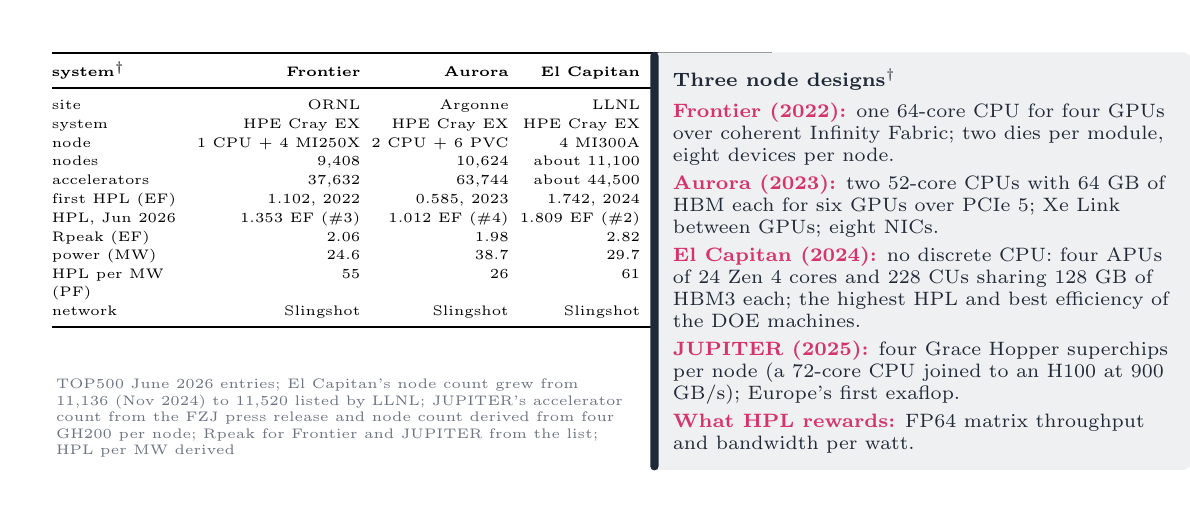
\begin{tikzpicture}
  \useasboundingbox (0,0) rectangle (14.4,5.9);
  \node[anchor=north west,inner sep=0,font=\fontsize{5.4}{6.4}\selectfont] at (0.3,5.6) {%
    \renewcommand{\arraystretch}{1.06}\setlength{\tabcolsep}{2.0pt}%
    \begin{tabular}{@{}>{\raggedright\arraybackslash}p{1.7cm}rrrr@{}}
      \toprule
      \textbf{system}$^\dagger$ & \textbf{Frontier} & \textbf{Aurora} & \textbf{El Capitan} & \textbf{JUPITER}\\
      \midrule
      site & ORNL & Argonne & LLNL & J\"ulich\\
      system & HPE Cray EX & HPE Cray EX & HPE Cray EX & BullSequana\\
      node & 1 CPU $+$ 4 MI250X & 2 CPU $+$ 6 PVC & 4 MI300A & 4 GH200\\
      nodes & 9{,}408 & 10{,}624 & about 11{,}100 & about 6{,}000\\
      accelerators & 37{,}632 & 63{,}744 & about 44{,}500 & about 24{,}000\\
      first HPL (EF) & 1.102, 2022 & 0.585, 2023 & 1.742, 2024 & 0.793, 2025\\
      HPL, Jun 2026 & 1.353 EF (\#3) & 1.012 EF (\#4) & 1.809 EF (\#2) & 1.000 EF (\#5)\\
      Rpeak (EF) & 2.06 & 1.98 & 2.82 & 1.23\\
      power (MW) & 24.6 & 38.7 & 29.7 & 15.8\\
      HPL per MW (PF) & 55 & 26 & 61 & 63\\
      network & Slingshot & Slingshot & Slingshot & InfiniBand\\
      \bottomrule
    \end{tabular}};
  \node[lab,font=\tiny,anchor=north west,text width=7.2cm,align=flush left] at (0.3,1.5) {TOP500 June 2026 entries; El Capitan's node count grew from 11,136 (Nov 2024) to 11,520 listed by LLNL; JUPITER's accelerator count from the FZJ press release and node count derived from four GH200 per node; Rpeak for Frontier and JUPITER from the list; HPL per MW derived};
  \bgpanels{7.9}{5.6}{6.3cm}{Three node designs$^\dagger$}{%
    \hl{outc}{Frontier (2022):} one 64-core CPU for four GPUs over
    coherent Infinity Fabric; two dies per module, eight devices per
    node.\\[2pt]
    \hl{outc}{Aurora (2023):} two 52-core CPUs with 64 GB of HBM each
    for six GPUs over PCIe 5; Xe Link between GPUs; eight NICs.\\[2pt]
    \hl{outc}{El Capitan (2024):} no discrete CPU: four APUs of 24 Zen
    4 cores and 228 CUs sharing 128 GB of HBM3 each; the highest HPL
    and best efficiency of the DOE machines.\\[2pt]
    \hl{outc}{JUPITER (2025):} four Grace Hopper superchips per node
    (a 72-core CPU joined to an H100 at 900 GB/s); Europe's first
    exaflop.\\[2pt]
    \hl{outc}{What HPL rewards:} FP64 matrix throughput and bandwidth
    per watt.}
\end{tikzpicture}
\end{frame}

% ---------------------------------------------------------------- 28
\begin{frame}{TOP500 and Green500, June 2026: who runs what}
\framesubtitle{A CPU-only Chinese system leads; AMD holds four of the top eight; the four most efficient are Grace Hopper.}
\centering
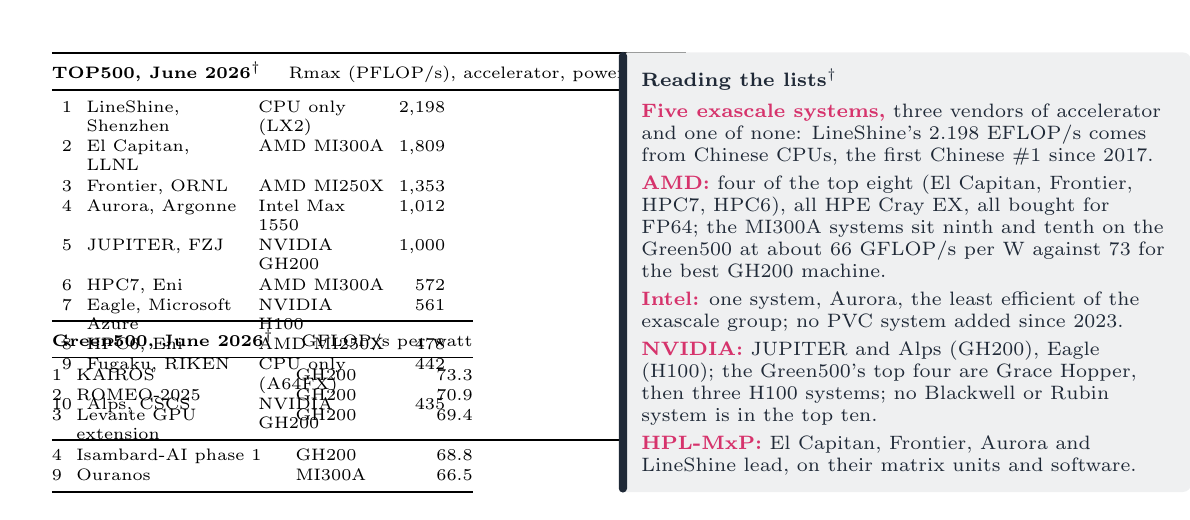
\begin{tikzpicture}
  \useasboundingbox (0,0) rectangle (14.4,5.9);
  \node[anchor=north west,inner sep=0,font=\fontsize{5.8}{6.9}\selectfont] at (0.3,5.6) {%
    \renewcommand{\arraystretch}{1.06}\setlength{\tabcolsep}{2.6pt}%
    \begin{tabular}{@{}r>{\raggedright\arraybackslash}p{2.0cm}>{\raggedright\arraybackslash}p{1.6cm}rr@{}}
      \toprule
      \multicolumn{5}{@{}l@{}}{\textbf{TOP500, June 2026}$^\dagger$ \quad Rmax (PFLOP/s), accelerator, power (MW)}\\
      \midrule
      1 & LineShine, Shenzhen & CPU only (LX2) & 2{,}198 & 42.2\\
      2 & El Capitan, LLNL & AMD MI300A & 1{,}809 & 29.7\\
      3 & Frontier, ORNL & AMD MI250X & 1{,}353 & 24.6\\
      4 & Aurora, Argonne & Intel Max 1550 & 1{,}012 & 38.7\\
      5 & JUPITER, FZJ & NVIDIA GH200 & 1{,}000 & 15.8\\
      6 & HPC7, Eni & AMD MI300A & 572 & 8.7\\
      7 & Eagle, Microsoft Azure & NVIDIA H100 & 561 & ---\\
      8 & HPC6, Eni & AMD MI250X & 478 & 8.5\\
      9 & Fugaku, RIKEN & CPU only (A64FX) & 442 & 29.9\\
      10 & Alps, CSCS & NVIDIA GH200 & 435 & 7.1\\
      \bottomrule
    \end{tabular}};
  \node[anchor=north west,inner sep=0,font=\fontsize{5.8}{6.9}\selectfont] at (0.3,2.2) {%
    \renewcommand{\arraystretch}{1.06}\setlength{\tabcolsep}{2.6pt}%
    \begin{tabular}{@{}r>{\raggedright\arraybackslash}p{2.6cm}>{\raggedright\arraybackslash}p{1.6cm}r@{}}
      \toprule
      \multicolumn{4}{@{}l@{}}{\textbf{Green500, June 2026}$^\dagger$ \quad GFLOP/s per watt}\\
      \midrule
      1 & KAIROS & GH200 & 73.3\\
      2 & ROMEO-2025 & GH200 & 70.9\\
      3 & Levante GPU extension & GH200 & 69.4\\
      4 & Isambard-AI phase 1 & GH200 & 68.8\\
      9 & Ouranos & MI300A & 66.5\\
      \bottomrule
    \end{tabular}};
  \bgpanels{7.5}{5.6}{6.7cm}{Reading the lists$^\dagger$}{%
    \hl{outc}{Five exascale systems,} three vendors of accelerator
    and one of none: LineShine's 2.198 EFLOP/s comes from Chinese
    CPUs, the first Chinese \#1 since 2017.\\[2pt]
    \hl{outc}{AMD:} four of the top eight (El Capitan, Frontier, HPC7,
    HPC6), all HPE Cray EX, all bought for FP64; the MI300A systems
    sit ninth and tenth on the Green500 at about 66 GFLOP/s per W
    against 73 for the best GH200 machine.\\[2pt]
    \hl{outc}{Intel:} one system, Aurora, the least efficient of the
    exascale group; no PVC system added since 2023.\\[2pt]
    \hl{outc}{NVIDIA:} JUPITER and Alps (GH200), Eagle (H100); the
    Green500's top four are Grace Hopper, then three H100 systems; no
    Blackwell or Rubin system is in the top ten.\\[2pt]
    \hl{outc}{HPL-MxP:} El Capitan, Frontier, Aurora and LineShine
    lead, on their matrix units and software.}
\end{tikzpicture}
\end{frame}

% ---------------------------------------------------------------- 29
\begin{frame}{The next machines and the gigawatt deals}
\framesubtitle{DOE's 2026--28 systems split three ways; the AI commitments of 2025--26 are measured in gigawatts, not GPUs.}
\centering
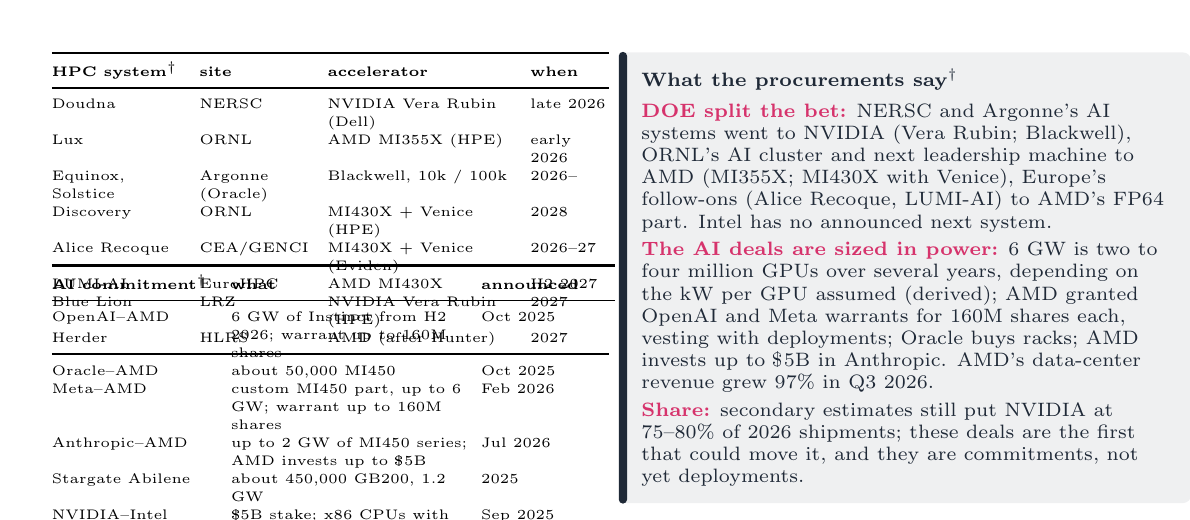
\begin{tikzpicture}
  \useasboundingbox (0,0) rectangle (14.4,5.9);
  \node[anchor=north west,inner sep=0,font=\fontsize{5.5}{6.5}\selectfont] at (0.3,5.6) {%
    \renewcommand{\arraystretch}{1.0}\setlength{\tabcolsep}{2.5pt}%
    \begin{tabular}{@{}>{\raggedright\arraybackslash}p{1.7cm}>{\raggedright\arraybackslash}p{1.45cm}>{\raggedright\arraybackslash}p{2.4cm}>{\raggedright\arraybackslash}p{1.0cm}@{}}
      \toprule
      \textbf{HPC system}$^\dagger$ & \textbf{site} & \textbf{accelerator} & \textbf{when}\\
      \midrule
      Doudna & NERSC & NVIDIA Vera Rubin (Dell) & late 2026\\
      Lux & ORNL & AMD MI355X (HPE) & early 2026\\
      Equinox, Solstice & Argonne (Oracle) & Blackwell, 10k / 100k & 2026--\\
      Discovery & ORNL & MI430X $+$ Venice (HPE) & 2028\\
      Alice Recoque & CEA/GENCI & MI430X $+$ Venice (Eviden) & 2026--27\\
      LUMI-AI & EuroHPC & AMD MI430X & H2 2027\\
      Blue Lion & LRZ & NVIDIA Vera Rubin (HPE) & 2027\\
      Herder & HLRS & AMD (after Hunter) & 2027\\
      \bottomrule
    \end{tabular}};
  \node[anchor=north west,inner sep=0,font=\fontsize{5.5}{6.5}\selectfont] at (0.3,2.9) {%
    \renewcommand{\arraystretch}{1.0}\setlength{\tabcolsep}{2.5pt}%
    \begin{tabular}{@{}>{\raggedright\arraybackslash}p{2.1cm}>{\raggedright\arraybackslash}p{3.0cm}>{\raggedright\arraybackslash}p{1.7cm}@{}}
      \toprule
      \textbf{AI commitment}$^\dagger$ & \textbf{what} & \textbf{announced}\\
      \midrule
      OpenAI--AMD & 6 GW of Instinct from H2 2026; warrant up to 160M shares & Oct 2025\\
      Oracle--AMD & about 50{,}000 MI450 & Oct 2025\\
      Meta--AMD & custom MI450 part, up to 6 GW; warrant up to 160M shares & Feb 2026\\
      Anthropic--AMD & up to 2 GW of MI450 series; AMD invests up to \$5B & Jul 2026\\
      Stargate Abilene & about 450{,}000 GB200, 1.2 GW & 2025\\
      NVIDIA--Intel & \$5B stake; x86 CPUs with NVLink & Sep 2025\\
      \bottomrule
    \end{tabular}};
  \bgpanels{7.5}{5.6}{6.7cm}{What the procurements say$^\dagger$}{%
    \hl{outc}{DOE split the bet:} NERSC and Argonne's AI systems went
    to NVIDIA (Vera Rubin; Blackwell), ORNL's AI cluster and next
    leadership machine to AMD (MI355X; MI430X with Venice), Europe's
    follow-ons (Alice Recoque, LUMI-AI) to AMD's FP64 part. Intel has
    no announced next system.\\[2pt]
    \hl{outc}{The AI deals are sized in power:} 6 GW is two to four
    million GPUs over several years, depending on the kW per GPU
    assumed (derived); AMD granted OpenAI and Meta warrants for 160M
    shares each, vesting with deployments; Oracle buys racks; AMD
    invests up to \$5B in Anthropic. AMD's data-center revenue grew
    97\% in Q3 2026.\\[2pt]
    \hl{outc}{Share:} secondary estimates still put NVIDIA at
    75--80\% of 2026 shipments; these deals are the first that could
    move it, and they are commitments, not yet deployments.}
\end{tikzpicture}
\end{frame}

% ---------------------------------------------------------------- 30
\stage{9}
\begin{frame}{MLPerf: where AMD and NVIDIA meet on the same benchmark}
\framesubtitle{AMD entered in 2024 (inference) and 2025 (training); by 2026 the MI355X trades blows with the B200.}
\centering
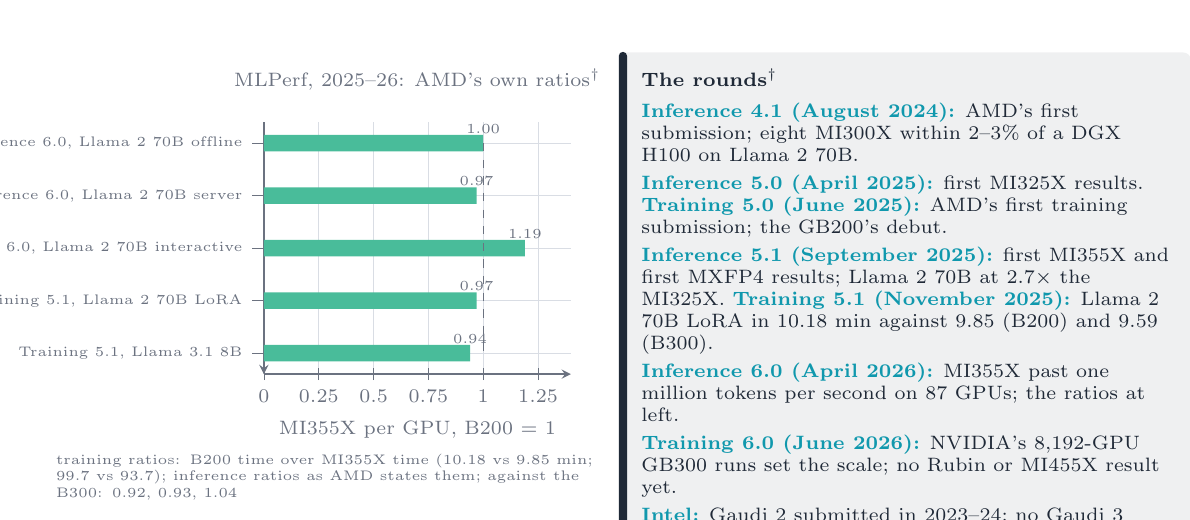
\begin{tikzpicture}
  \useasboundingbox (0,0) rectangle (14.4,5.9);
  \begin{scope}[shift={(3.0,1.5)}]
  \begin{axis}[lecture,scale only axis,width=3.9cm,height=3.2cm,xbar,bar width=6pt,xmin=0,xmax=1.4,enlarge y limits=0.1,
      symbolic y coords={{Inference 6.0, Llama 2 70B offline},{Inference 6.0, Llama 2 70B server},{Inference 6.0, Llama 2 70B interactive},{Training 5.1, Llama 2 70B LoRA},{Training 5.1, Llama 3.1 8B}},
      ytick=data,y dir=reverse,yticklabel style={font=\tiny},xlabel={MI355X per GPU, B200 $=$ 1},
      xtick={0,0.25,0.5,0.75,1,1.25},
      nodes near coords,nodes near coords style={font=\tiny,text=muted},point meta=explicit symbolic,
      title style={font=\scriptsize,text=muted,at={(0.5,1.02)}},title={MLPerf, 2025--26: AMD's own ratios$^\dagger$}]
    \addplot[fill=emb!75,draw=none] coordinates {(1.0,{Inference 6.0, Llama 2 70B offline})[1.00] (0.97,{Inference 6.0, Llama 2 70B server})[0.97] (1.19,{Inference 6.0, Llama 2 70B interactive})[1.19] (0.97,{Training 5.1, Llama 2 70B LoRA})[0.97] (0.94,{Training 5.1, Llama 3.1 8B})[0.94]};
    \draw[muted,dashed] (axis cs:1,{Inference 6.0, Llama 2 70B offline}) -- (axis cs:1,{Training 5.1, Llama 3.1 8B});
  \end{axis}
  \end{scope}
  \node[lab,font=\tiny,anchor=north west,text width=7.2cm] at (0.3,0.55) {training ratios: B200 time over MI355X time (10.18 vs 9.85 min; 99.7 vs 93.7); inference ratios as AMD states them; against the B300: 0.92, 0.93, 1.04};
  \bgpanels{7.5}{5.6}{6.7cm}{The rounds$^\dagger$}{%
    \hl{vc}{Inference 4.1 (August 2024):} AMD's first submission; eight
    MI300X within 2--3\% of a DGX H100 on Llama 2 70B.\\[2pt]
    \hl{vc}{Inference 5.0 (April 2025):} first MI325X results.
    \hl{vc}{Training 5.0 (June 2025):} AMD's first training
    submission; the GB200's debut.\\[2pt]
    \hl{vc}{Inference 5.1 (September 2025):} first MI355X and first
    MXFP4 results; Llama 2 70B at 2.7$\times$ the MI325X.
    \hl{vc}{Training 5.1 (November 2025):} Llama 2 70B LoRA in 10.18
    min against 9.85 (B200) and 9.59 (B300).\\[2pt]
    \hl{vc}{Inference 6.0 (April 2026):} MI355X past one million
    tokens per second on 87 GPUs; the ratios at left.\\[2pt]
    \hl{vc}{Training 6.0 (June 2026):} NVIDIA's 8{,}192-GPU GB300
    runs set the scale; no Rubin or MI455X result yet.\\[2pt]
    \hl{vc}{Intel:} Gaudi 2 submitted in 2023--24; no Gaudi 3
    submission on record.}
\end{tikzpicture}
\end{frame}

% ---------------------------------------------------------------- 31
\stage{10}
\begin{frame}{The platforms in one table}
\framesubtitle{Seven accelerators from three vendors, 2023--2026, as their datasheets state them.}
\centering
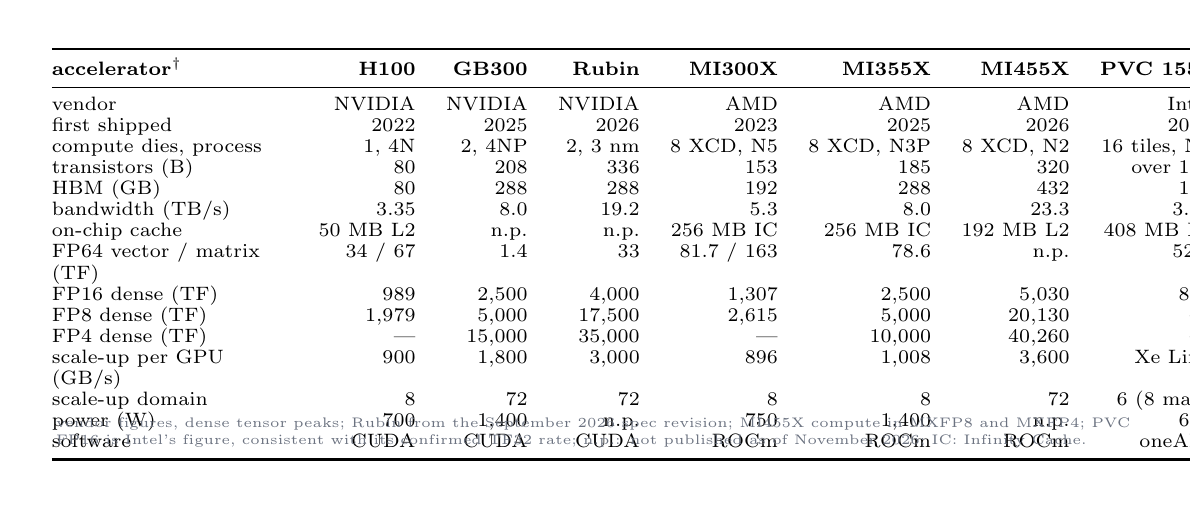
\begin{tikzpicture}
  \useasboundingbox (0,0) rectangle (14.4,5.9);
  \node[anchor=north west,inner sep=0,font=\fontsize{6.6}{7.6}\selectfont] at (0.3,5.65) {%
    \renewcommand{\arraystretch}{1.0}\setlength{\tabcolsep}{5.5pt}%
    \begin{tabular}{@{}>{\raggedright\arraybackslash}p{3.0cm}rrrrrrr@{}}
      \toprule
      \textbf{accelerator}$^\dagger$ & \textbf{H100} & \textbf{GB300} & \textbf{Rubin} & \textbf{MI300X} & \textbf{MI355X} & \textbf{MI455X} & \textbf{PVC 1550}\\
      \midrule
      vendor & NVIDIA & NVIDIA & NVIDIA & AMD & AMD & AMD & Intel\\
      first shipped & 2022 & 2025 & 2026 & 2023 & 2025 & 2026 & 2023\\
      compute dies, process & 1, 4N & 2, 4NP & 2, 3 nm & 8 XCD, N5 & 8 XCD, N3P & 8 XCD, N2 & 16 tiles, N5\\
      transistors (B) & 80 & 208 & 336 & 153 & 185 & 320 & over 100\\
      HBM (GB) & 80 & 288 & 288 & 192 & 288 & 432 & 128\\
      bandwidth (TB/s) & 3.35 & 8.0 & 19.2 & 5.3 & 8.0 & 23.3 & 3.28\\
      on-chip cache & 50 MB L2 & n.p. & n.p. & 256 MB IC & 256 MB IC & 192 MB L2 & 408 MB L2\\
      FP64 vector / matrix (TF) & 34 / 67 & 1.4 & 33 & 81.7 / 163 & 78.6 & n.p. & 52.4\\
      FP16 dense (TF) & 989 & 2{,}500 & 4{,}000 & 1{,}307 & 2{,}500 & 5{,}030 & 839\\
      FP8 dense (TF) & 1{,}979 & 5{,}000 & 17{,}500 & 2{,}615 & 5{,}000 & 20{,}130 & ---\\
      FP4 dense (TF) & --- & 15{,}000 & 35{,}000 & --- & 10{,}000 & 40{,}260 & ---\\
      scale-up per GPU (GB/s) & 900 & 1{,}800 & 3{,}000 & 896 & 1{,}008 & 3{,}600 & Xe Link\\
      scale-up domain & 8 & 72 & 72 & 8 & 8 & 72 & 6 (8 max)\\
      power (W) & 700 & 1{,}400 & n.p. & 750 & 1{,}400 & n.p. & 600\\
      software & CUDA & CUDA & CUDA & ROCm & ROCm & ROCm & oneAPI\\
      \bottomrule
    \end{tabular}};
  \node[lab,anchor=north west,text width=13.8cm,font=\tiny] at (0.3,1.0) {vendor figures, dense tensor peaks; Rubin from the September 2026 spec revision; MI455X compute in MXFP8 and MXFP4; PVC FP16 is Intel's figure, consistent with its confirmed TF32 rate; n.p.: not published as of November 2026; IC: Infinity Cache.};
\end{tikzpicture}
\end{frame}

% ---------------------------------------------------------------- 32
\begin{frame}{Summary: what to take from this lecture}
\framesubtitle{The dies converged, the platforms did not; the fabric, the software and the buying model decide.}
\centering
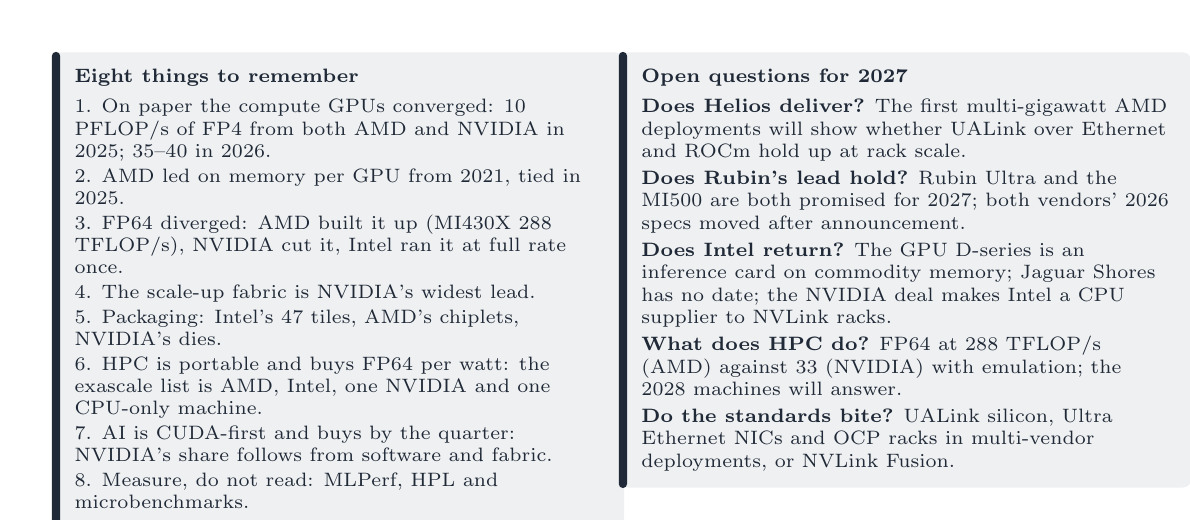
\begin{tikzpicture}
  \useasboundingbox (0,0) rectangle (14.4,5.9);
  \bgpanels{0.3}{5.6}{6.7cm}{Eight things to remember}{%
    1. On paper the compute GPUs converged: 10 PFLOP/s of FP4 from
    both AMD and NVIDIA in 2025; 35--40 in 2026.\\[1pt]
    2. AMD led on memory per GPU from 2021, tied in 2025.\\[1pt]
    3. FP64 diverged: AMD built it up (MI430X 288 TFLOP/s), NVIDIA
    cut it, Intel ran it at full rate once.\\[1pt]
    4. The scale-up fabric is NVIDIA's widest lead.\\[1pt]
    5. Packaging: Intel's 47 tiles, AMD's chiplets, NVIDIA's dies.\\[1pt]
    6. HPC is portable and buys FP64 per watt: the exascale list is
    AMD, Intel, one NVIDIA and one CPU-only machine.\\[1pt]
    7. AI is CUDA-first and buys by the quarter: NVIDIA's share
    follows from software and fabric.\\[1pt]
    8. Measure, do not read: MLPerf, HPL and microbenchmarks.}
  \bgpanels{7.5}{5.6}{6.7cm}{Open questions for 2027}{%
    \hl{ink}{Does Helios deliver?} The first multi-gigawatt AMD
    deployments will show whether UALink over Ethernet and ROCm hold
    up at rack scale.\\[2pt]
    \hl{ink}{Does Rubin's lead hold?} Rubin Ultra and the MI500 are
    both promised for 2027; both vendors' 2026 specs moved after
    announcement.\\[2pt]
    \hl{ink}{Does Intel return?} The GPU D-series is an inference card
    on commodity memory; Jaguar Shores has no date; the NVIDIA deal
    makes Intel a CPU supplier to NVLink racks.\\[2pt]
    \hl{ink}{What does HPC do?} FP64 at 288 TFLOP/s (AMD) against 33
    (NVIDIA) with emulation; the 2028 machines will answer.\\[2pt]
    \hl{ink}{Do the standards bite?} UALink silicon, Ultra Ethernet
    NICs and OCP racks in multi-vendor deployments, or NVLink Fusion.}
\end{tikzpicture}
\end{frame}

% ---------------------------------------------------------------- 33
\begin{frame}{Sources}
\framesubtitle{Whitepapers and datasheets, papers and talks, lists and reporting; $^\dagger$ marks vendor material.}
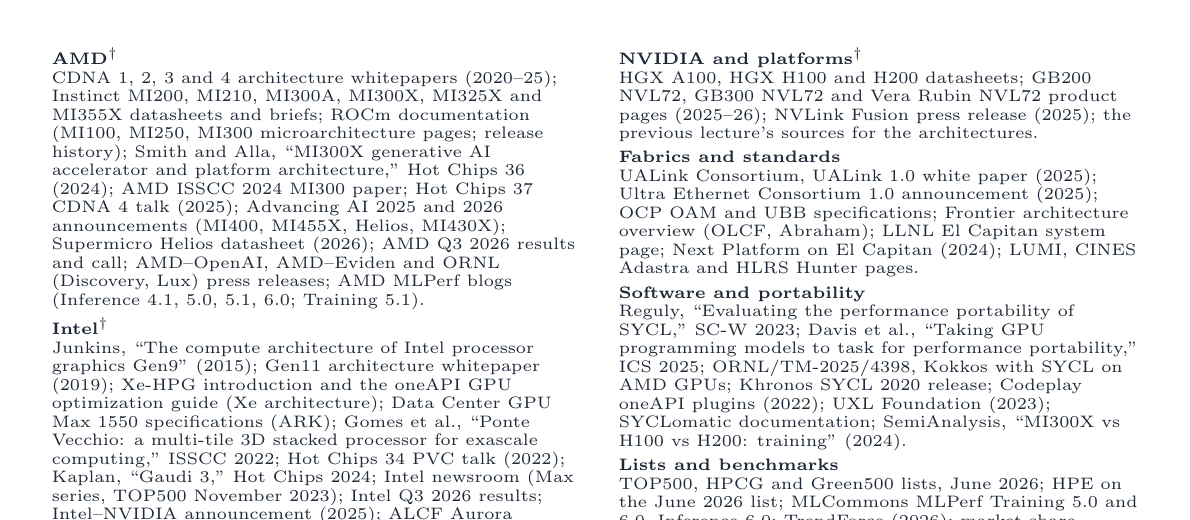
\begin{tikzpicture}
  \useasboundingbox (0,0) rectangle (14.4,5.9);
  \node[anchor=north west,inner sep=0,text width=6.8cm,font=\fontsize{5.6}{6.7}\selectfont,text=ink,align=flush left] at (0.3,5.65) {%
    \textbf{AMD}$^\dagger$\\
    CDNA 1, 2, 3 and 4 architecture whitepapers (2020--25); Instinct MI200, MI210, MI300A, MI300X, MI325X and MI355X datasheets and briefs; ROCm documentation (MI100, MI250, MI300 microarchitecture pages; release history); Smith and Alla, ``MI300X generative AI accelerator and platform architecture,'' Hot Chips 36 (2024); AMD ISSCC 2024 MI300 paper; Hot Chips 37 CDNA 4 talk (2025); Advancing AI 2025 and 2026 announcements (MI400, MI455X, Helios, MI430X); Supermicro Helios datasheet (2026); AMD Q3 2026 results and call; AMD--OpenAI, AMD--Eviden and ORNL (Discovery, Lux) press releases; AMD MLPerf blogs (Inference 4.1, 5.0, 5.1, 6.0; Training 5.1).\\[2pt]
    \textbf{Intel}$^\dagger$\\
    Junkins, ``The compute architecture of Intel processor graphics Gen9'' (2015); Gen11 architecture whitepaper (2019); Xe-HPG introduction and the oneAPI GPU optimization guide (Xe architecture); Data Center GPU Max 1550 specifications (ARK); Gomes et al., ``Ponte Vecchio: a multi-tile 3D stacked processor for exascale computing,'' ISSCC 2022; Hot Chips 34 PVC talk (2022); Kaplan, ``Gaudi 3,'' Hot Chips 2024; Intel newsroom (Max series, TOP500 November 2023); Intel Q3 2026 results; Intel--NVIDIA announcement (2025); ALCF Aurora documentation; Goto et al., ``HPL and HPL-MxP at exascale on Aurora'' (2026); Hatanp\"a\"a et al., AERIS (2025); HPCwire, ``Aurora the survivor'' (2023); reporting on Rialto Bridge, Falcon Shores, Crescent Island and the GPU D-series.};
  \node[anchor=north west,inner sep=0,text width=6.6cm,font=\fontsize{5.6}{6.7}\selectfont,text=ink,align=flush left] at (7.5,5.65) {%
    \textbf{NVIDIA and platforms}$^\dagger$\\
    HGX A100, HGX H100 and H200 datasheets; GB200 NVL72, GB300 NVL72 and Vera Rubin NVL72 product pages (2025--26); NVLink Fusion press release (2025); the previous lecture's sources for the architectures.\\[2pt]
    \textbf{Fabrics and standards}\\
    UALink Consortium, UALink 1.0 white paper (2025); Ultra Ethernet Consortium 1.0 announcement (2025); OCP OAM and UBB specifications; Frontier architecture overview (OLCF, Abraham); LLNL El Capitan system page; Next Platform on El Capitan (2024); LUMI, CINES Adastra and HLRS Hunter pages.\\[2pt]
    \textbf{Software and portability}\\
    Reguly, ``Evaluating the performance portability of SYCL,'' SC-W 2023; Davis et al., ``Taking GPU programming models to task for performance portability,'' ICS 2025; ORNL/TM-2025/4398, Kokkos with SYCL on AMD GPUs; Khronos SYCL 2020 release; Codeplay oneAPI plugins (2022); UXL Foundation (2023); SYCLomatic documentation; SemiAnalysis, ``MI300X vs H100 vs H200: training'' (2024).\\[2pt]
    \textbf{Lists and benchmarks}\\
    TOP500, HPCG and Green500 lists, June 2026; HPE on the June 2026 list; MLCommons MLPerf Training 5.0 and 6.0, Inference 6.0; TrendForce (2026); market-share estimates (Silicon Analysts, 2026; secondary). Full list with links in the paper kit.};
\end{tikzpicture}
\end{frame}
\end{document}
